\documentclass[11pt]{article}

% preamble
\usepackage{graphicx}
\usepackage[nottoc,numbib]{tocbibind}
\usepackage{tabularx}
\usepackage[parfill]{parskip}
\usepackage{amsmath}
\usepackage[hyphens]{url}
\usepackage[table]{xcolor}
\definecolor{skyblue}{HTML}{3366cc}
\usepackage[hidelinks, colorlinks=true, linkcolor=black, urlcolor=skyblue, citecolor=skyblue, allcolors=skyblue]{hyperref}
\usepackage{fancyhdr}
\usepackage{titlesec}
\usepackage{listings}
\usepackage[acronym]{glossaries}
\usepackage[all]{hypcap}
\usepackage{textcomp}
\usepackage{url}
\usepackage{attachfile}
\usepackage[super]{natbib}
\usepackage{float}
%\usepackage[czech]{babel}

%\hypersetup{colorlinks=true, pdfstartview=FitV, linkcolor=blue, citecolor=black, plainpages=false, pdfpagelabels=true, urlcolor=blue}

\setcitestyle{square}

\definecolor{codegreen}{rgb}{0,0.6,0}
\definecolor{codegray}{rgb}{0.5,0.5,0.5}
\definecolor{codepurple}{rgb}{0.58,0,0.82}
\definecolor{backcolour}{rgb}{1.0, 1.0, 1.0}
\lstdefinestyle{mystyle}{
    backgroundcolor=\color{backcolour},   
    commentstyle=\color{codegreen},
    keywordstyle=\color{blue},
    numberstyle=\tiny\color{codegray},
    stringstyle=\color{codepurple},
    basicstyle=\ttfamily\footnotesize,
    breakatwhitespace=false,         
    breaklines=true,                 
    captionpos=b,                    
    keepspaces=true,                 
    numbers=left,                    
    numbersep=5pt,                  
    showspaces=false,                
    showstringspaces=false,
    showtabs=false,                  
    tabsize=4
}
\lstset{style=mystyle}
\setcounter{secnumdepth}{5}

\makenoidxglossaries

\newglossaryentry{vulkan}{name=Vulkan, description={Low-level GPU application programmable interface}}
\newglossaryentry{cpp}{name=C++,description={Low-level programming language}}
\newglossaryentry{cl}{name=CL,description={The Microsoft C compiler and linker}}
\newglossaryentry{msbuild}{name=MSBuild,description={Microsoft project build system}}

\setacronymstyle{long-short}
\newacronym{cpu}{CPU}{Central Processing Unit}
\newacronym{os}{OS}{Operating System}
\newacronym{gpu}{GPU}{Graphics Processing Unit}
\newacronym{ram}{RAM}{Random Access Memory}
\newacronym{vram}{VRAM}{Video Random Access Memory}
\newacronym{wsi}{WSI}{Window System Integration}
\newacronym{aes}{AES}{Advanced Encryption Standard}
\newacronym{glsl}{GLSL}{OpenGL Shading Language}
\newacronym{lib}{LIB}{Static Library}
\newacronym{dll}{DLL}{Dynamic Link Library}
\newacronym{pch}{PCH}{Precompiled Header}
\newacronym{cli}{CLI}{Command Line Interface}
\newacronym{vmve}{VMVE}{Vulkan Model Viewer and Exporter}
\newacronym{api}{API}{Application Programmable Interface}
\newacronym{exe}{EXE}{Windows Executable}
\newacronym{vma}{VMA}{Vulkan Memory Allocator}
\newacronym{ide}{IDE}{Integrated Development Environment}
\newacronym{vcs}{VCS}{Version Control System}
\newacronym{msvc}{MSVC}{Microsoft Visual Compiler}
\newacronym{stl}{STL}{C++ Standard Template Library}
\newacronym{lod}{LOD}{Level of Detail}
\newacronym{ip}{IP}{Intellectual Property}
\newacronym{ui}{UI}{User Interface}
\newacronym{gdpr}{GDPR}{General Data Protection Regulation}
\newacronym{svn}{SVN}{Apache Subversion}

% end of preamble

% document
\pagenumbering{gobble}

\begin{document}

\hypersetup{
  pdftitle={Optimizing workflow for virtual environments using Vulkan Model Viewer and Exporter},
  pdfsubject={Computer Graphics},
  pdfauthor={Zakariya Oulhadj},
  pdfkeywords={vmve, graphics, vulkan, report, game engine, rendering}
}

\begin{titlepage}
	\centering
  
\includegraphics[scale=0.35]{images/university-logo.png}\par
  \vspace{1cm}
	{\huge\textbf{Optimizing workflow for virtual environments using Vulkan Model Viewer and Exporter}\par}
  \vspace{1cm}
  The University of Roehampton\\
  Department of Arts and Digital Industries\\
  London, United Kingdom
  \vspace{1cm}
  \vfill
  \begin{minipage}[t]{0.4\textwidth}
		\begin{flushleft}
			\large
			\textit{Author}\\
			Mr. \textsc{Zakariya Oulhadj} % Your name
		\end{flushleft}
	\end{minipage}
	~
	\begin{minipage}[t]{0.4\textwidth}
		\begin{flushright}
			\large
			\textit{Supervisors}\\
			Dr. \textsc{Charles Clarke} % Supervisor's name
      \textsc{Alex Collins} % Supervisor's name
		\end{flushright}
	\end{minipage}

  \vfill
  Submitted in partial fulfillment of the requirements for the degree of \\
  \textit{Bachelors of Science in Computer Science}
  \vfill
	{\large \today\par}
\end{titlepage}

\pagebreak
\pagestyle{empty}


\begin{center}
\thispagestyle{empty}  
\vspace*{\fill}
\textit{This report is dedicated to my family, friends and lecturers who have supported me throughout my degree}
\vspace*{\fill}
\end{center}


\pagebreak

\section*{Abstract}
Computer graphics is a rapidly growing field that is vital in many industries
that rely on digital graphics including scientific research, simulations,
education and training, entertainment and more. The flexibility and increase of
computing resources provide real-world benefits in ways not previously observed
before the use of computer imagery.

This report presents my final year project an application built using the latest
technologies as a learning tool for 3D model rendering. Its goal is to be easy
to use, performant and provide a collection of tools for graphics manipulation
that users can take advantage of when designing and building virtual
environments. It's intended to serve as an important application that bridges
the gap between inexperienced users and industry-leading rendering engines.

\pagebreak

\section*{Declaration}
I hereby certify that this report constitutes my work, that where the language
of others is used, quotation marks so indicate, and that appropriate credit is
given where I have used the language, ideas, expressions, or writings of others.
I declare that this report describes the original work that has not been
previously presented for the award of any other degree or institution.

\noindent
\begin{tabular}[b]{@{} p{6cm} @{}}
\today \\
\hline
\scriptsize Date
\end{tabular}\qquad
\begin{tabular}[b]{@{} p{6cm} @{}}

\includegraphics[width=6cm,height=1cm]{images/signature.png} \\
\hline
\scriptsize Signature
\end{tabular}

\pagebreak
{
  \hypersetup{linkcolor=black}
  \tableofcontents
  \addtocontents{toc}{~\hfill\textbf{Page}\par}
}
\pagebreak

\clearpage
\printnoidxglossary[nonumberlist]

\clearpage
\printnoidxglossary[type=\acronymtype, nonumberlist]

\pagebreak
\pagestyle{fancy}
\pagenumbering{arabic}

\section{Introduction}
Computer graphics is a vast area within the field of Computer Science. Since its
conception in the early 1960s, it has been used for a wide range of purposes
including gaming, film, scientific research, education, architecture,
engineering, medicine and more recently within vehicles. This is a testament to
how versatile this field has become and consists of numerous benefits that
computer graphics provide to the real world.

\subsection{Project Problem}
Industrial graphics software today are large and highly technical applications
that are the culmination of decades worth of work. Examples include Unreal
Engine \cite{unreal_engine}, Unity \cite{unity} and RenderMan \cite{render_man}.
These applications provide users with innovative technologies such as ray tracing,
real-time global illumination, subsurface scattering, geometry compression,
streaming and much more that are designed for use in professional environments
which results in stringent requirements and complex feature sets.

This results in the adoption of the software being a barrier to entry for
graphics developers, artists and businesses which inadvertently introduces a
wide range of issues such as requiring training for employees, additional costs
for businesses and a decrease in productivity. Other issues include performance,
compatibility and storage when using these complex applications.

% todo: back this up with data/from a paper

To address these issues, I introduce my final year project, \gls*{vmve}. A
standalone application developed in the domain of computer graphics that
provides an easy-to-use, efficient platform for 3D graphics rendering and asset
encryption. It will also serve as an important tool and as a stepping stone that
aims to bridge to gap between new users and industry-leading rendering engines.

To achieve this, \gls*{vmve} will provide a small but specific subset of
features that are designed from the ground up to be easy to use and understand
for rapid graphics prototyping such as constructing virtual environments,
simulating the effect of light on 3D geometry and securing digital assets
through the use of encryption.

\subsection{Stakeholders} \label{stakeholders}
Stakeholders are individuals or groups who have an interest or "stake" in
\gls*{vmve} which can include decisions made throughout the development or the
end product. Each stakeholder group may have different goals, priorities, and
expectations, which can sometimes lead to conflicts and challenges in
decision-making and implementation. It is important to identify the different
groups to ensure their requirements and concerns are being taken into account so
that informed decisions can be made.

\subsubsection{Students and trainees}
Students and trainees are the key stakeholder groups for the project which the
application will be designed to accommodate by providing the necessary tools and
functionality. This includes providing a suite of easy-to-use tools for graphics
rendering that students and trainees could use to learn about basic rendering
concepts and to use this knowledge to construct virtual environments for
graphics prototyping and rendering.

\subsubsection{Businesses}
The other type of stakeholder is employers who will want to train new potential
employees in the field of computer graphics. The goal is for businesses to use
\gls*{vmve} as a training tool to lower the learning curve and reduce the
barrier to entry within the graphics industry.

\subsection{Requirements}
The design, implementation and evaluation of the project rely on a set of aims
and objectives to be fully defined. The first step toward obtaining these
requirements requires a ``requirements gathering'' stage. The purpose of this
is to outline and better understand the requirements for each of the
stakeholders mentioned in section \ref{stakeholders}.

\subsubsection{Aims} \label{aims} 

\gls*{vmve} has several aims which outline the general goals that the
application wishes to achieve throughout this project. These aims will go on to
define concrete objectives that provide a clear and concise set of instructions
required for the design and implementation stages.


\begin{description}
  \item[1. Virtual environment rendering] The first aim of \gls*{vmve} is to
    provide an ``easy-to-use'' platform for creating virtual environments. This
    means that the application should reduce the learning curve so that users
    with little to no prior experience with 3D rendering software and the
    underlying technology such as students and trainees can use the application
    to achieve their desired goals.

  \item[2. Lower system requirements] Many industry-leading applications are
    complex applications that have significant hardware requirements to run.
    \gls*{vmve} will aim to address this by focusing on the efficiency of the
    application and only providing the necessary tools needed which are not
    computationally expensive.

  \item[3. 3D asset encryption] The last of the three main aims is for the
    application to include a custom model format that makes use of encryption to
    safely secure a user's digital assets. The motivation for this functionality
    formed as a result of the increase in theft regarding digital assets. A
    recent example is the data leak that affected Rockstar Studios and their
    upcoming game (Grand Theft Auto 6) which saw assets, source code and
    documentation released to the public \cite{gta_leak}.

\end{description}


\subsubsection{Objectives} \label{objectives}
Fulfilling these aims requires a set of objectives i.e. requirements that need
to be implemented to achieve the aims outlined in section \ref{aims}.

\begin{description}
  \item[1. Virtual environment rendering] 
    The project will be built to run as a desktop application that renders a user
    interface editor as well as a virtual environment. The \gls*{ui} must be
    designed intuitively to reduce the amount of friction between the application
    and the user's goal. This means common related tasks and functionality must be
    grouped. Furthermore, the language used throughout the user interface must
    reduce if not eliminate jargon. Doing so will make the application easier to
    understand.

  \item[2. Lower system requirements]
    This can be achieved through the use of efficient technologies, algorithms
    and overall structure related to rendering that will allow for assets to be
    displayed using as few hardware resources as possible. For example, by
    using the latest rendering \glspl*{api} and packing/compressing crucial
    data. Efficiency requirements vary based on the component in question which
    includes the \gls*{cpu}, \gls*{gpu}, memory and storage. 


  \item[3. 3D asset encryption]
    \gls*{vmve} would be able to provide a platform to encrypt these assets and
    only unlock them using a special key that only the user will know. This
    ensures that in the event of digital assets begin obtained by third parties,
    they cannot be used. This requires several key elements to work in tandem to
    achieve this objective.
    
    The raw model must be able to be encrypted using different types of
    encryption algorithms. In addition to this, the application will need to
    include a parser that can read the internal structure of the encrypted file
    format and successfully load the model into the application.
\end{description}


% TODO: Should this be included?
With these aims and objectives fully defined, the project proposal document was signed off
as part of the requirements for milestone 2. 
\begin{figure}[H]
  \centering
  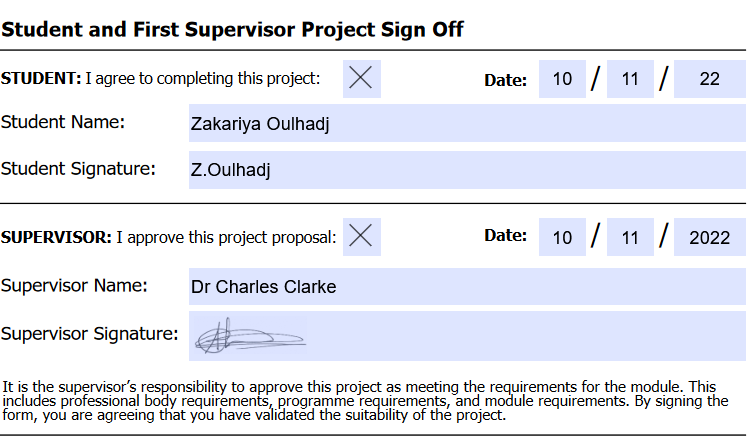
\includegraphics[width=\textwidth]{images/project_signoff.png}
  \caption{Project proposal sign-off}
  \label{fig:project_signoff}
\end{figure}

% The aims discussed above were part of the project proposal document and which
% was signed off for milestone 2. The complete document can be viewed in
% appendix section \ref{supporting_documents}.


\subsection{Considerations}
With the aims and objectives fully defined, important considerations must be
taken into account before commencing work on the application. These include
legal and ethical considerations.

\subsubsection{Legal}
The legality of \gls*{vmve} is one of the most important considerations that
must be taken into account. As the application is intended to be distributed to
users around the world, local laws and regulations must be adhered to. As a
relatively basic application that serves a specific user base, there is a small
set of features and functionality that require legal clarification.

\begin{description}
  \item[Encryption]
    Firstly, \gls*{vmve} will include the ability to secure critical assets such
    as 3D models. This will be achieved using encryption by making use of a
    secret key and initialisation vector. This information is not stored and is
    only generated once for a user to save in order to encrypt and decrypt a
    model.

  \item[Asset modification] 
    Secondly, \gls*{vmve} will not modify any of the raw data being imported and
    only change the visual appearance based on several factors including
    rendering settings, lighting, translation, rotation and scaling. 

  \item[Personal information] 
    Finally, the application does not store or process any personal information
    and will also not contain any networking functionality. This means that all
    data remains local to the application and the user's device. Therefore,
    \gls*{gdpr} will not need to be take into account. In the future, however,
    if the use of data and information changes then this will be revisited to
    ensure that all laws are adhered to. 
\end{description}

The source code for the project will not be publicly available throughout the
development. However, upon completion of the project, this may change and thus,
will be licensed under the MIT license \cite{mit} which states that the source
code can be used without restriction allowing for it to be copied, modified as
well as distributed.

\subsubsection{Ethical}
One of the main ethical considerations is the computation that the application
will perform internally. The technical implementation details are not accessible
to users as the source code is not open source. Therefore, individuals do not
know exactly what the software is doing during runtime.

To ensure that \gls*{vmve} remains ethical, the application will not perform any
additional computations that are not strictly required for 3D rendering.
Furthermore, the application will not store or send any data as this is not
required and would fall outside the scope of its initial aims and objectives.

Another ethical consideration is the use of deceptive design also known as
``Dark patterns'' that refers to designs/tricks that manipulate users into
performing certain actions without their informed consent. \gls*{vmve} will make
use of a user interface, however, during the design and implementation stages
extra effort will be spent on ensuring that no such design pattern is
introduced. This will greatly benefit users and their overall user experience.

\subsection{BSc Justification}
This project is ambitious and challenging that requires a strong understanding
of computer graphics, programming, and software architecture. It is a large
undertaking that uses the skills and knowledge gained through the BSc (Bachelor
of Science) computer science program from modules such as software development
(1, 2, 3), algorithms, data science, cybersecurity and mathematics. Not only
does it showcase technical ability but also highlights critical thinking,
problem-solving, decision-making and time management skills. As a result, they
will be highly valued in the professional industry and necessary for success in
the field of computer science and therefore, is a suitable choice for a
final-year project.

\subsection{Overview}
This report is structured such that it presents each aspect of the development
in chronological order. There are a total of four key sections in this report:
\begin{description}
  \item[Technology review (\ref{technology_review})] Covers the different
    technologies that could be potentially used throughout the development and
    outlines the advantages and disadvantages of each. This will lay the
    foundation for the design section.
  \item[Design (\ref{design})] Focuses on the concept of the project, the design
    of the requirements obtained during the requirements-gathering stage
    followed by the design of the application such as the tools going to be
    used, user interface and engine architecture.
  \item[Implementation (\ref{implementation})] Takes the proposed designs and
    consist of the development of the application as well as presenting the
    technical implementation details and decisions.
  \item[Conclusion (\ref{conclusion})] Reflects on the project to ensure that
    the application has met the aims and objectives originally set out and
    discusses the specific features that will need to be implemented going
    forward.
\end{description}

\clearpage
\section{Technology Review} \label{technology_review}
Prior to commencing work, a technological review must be undertaken that
analyses and compares different types of potential tools that could be used.
Throughout this comparison, the choice of potential tools is heavily influenced
by the aims and objectives outlined in sections \ref{aims} and \ref{objectives}
respectively.


\subsection{Version Control}
A \gls*{vcs} is a tool used for backing up and/or collaborating with developers
on a project. The use of a \gls*{vcs} was an obvious choice as this would
provide a platform on which the project source code could be hosted.
Furthermore, if for some reason a local copy of the project is lost or corrupted
then another copy is safely hosted on the servers managed by the \gls*{vcs}.

Another key feature of a \gls*{vcs} is project management. These types of
systems provide various tools that greatly benefit developers. One such feature
is known as a ``commit'' which records any changes made to a particular
repository at that moment in time. Developers use commits to view changes that
occur at each stage but also, provide means of reverting to previous versions of
particular sections, files or even an entire repository. Due to the length and
complexity of this project, tools such as this provided by a \gls*{vcs} are
invaluable throughout the development process. There are two main types of
systems, which are SVN and Git. 


\gls*{svn} was originally developed in 2000 by Apache and is a centralised
\gls*{vcs} which means that the repository is stored on a remote server which
developers all connect to.

On the other hand, Git is the most widely-used, free and open-source \gls*{vcs}
developed in 2005. It is a distributed system meaning that developers have
copies of a repository that they work off. Git is generally considered to be
faster and more efficient than \gls*{svn} as a result of its distributed
structure. Furthermore, Git is more flexible regarding how it can be
installed such as onto a server manually or by using existing platforms that are
built on top of Git. A few examples include \href{http://github.com}{GitHub},
\href{http://gitlab.com}{GitLab} and \href{https://bitbucket.org/}{Bitbucket}. 


According to the StackOverflow Developer Survey, in 2022 Git was the most widely used \gls*{vcs}
with an adoption percentage of 93.9\% as seen in figure \ref{fig:vcs_comparison}.
This shows how popular Git is compared to other similar systems \cite{vcs_survey}.

\begin{figure}[H]
\begin{center}
  \rowcolors{2}{gray!25}{white}
  \begin{tabular}{cc}
    
    \rowcolor{gray!50}
    Git & SVN \\
    93.9\% & 5.2\% \\
  \end{tabular}
\end{center}
\caption{Version control usage comparison}
\label{fig:vcs_comparison}
\end{figure}

\subsection{Development Environment}

The project will be developed using a dedicated development environment which is
a set of tools that provide helpful features. These features can include
debugging, formatting, source code analyses, profiling and much more.

\begin{description}
  \item[Microsoft Visual Studio 2022] This application is a fully-fledged
    \gls*{ide} that contains many different features that are dedicated to
    application development. In addition to the application, it comes with the
    \gls*{msvc} compiler which is Microsoft's own C/C++ compiler and linker.
    This is a program that parses source code and generates assembly
    instructions that the \gls*{cpu} will be able to understand and therefore,
    execute. The \gls*{ide} together with \gls*{msvc} create a solid ecosystem
    for development. The \gls*{ide} also provides debugging functionality that
    will be used extensively to fix crashes, and bugs and generally ensure that
    the application runs as expected \cite{visualstudio}. 

    The main downside to this option, however, is that it is only supported on
    the Windows operating system. Therefore, it's not available on macOS or
    Linux meaning that if the application will be cross-platform then other
    tools will be required.

  \item[Microsoft Visual Studio Code] Is a light and open-source text editor
    built using Electron which is flexible and has support for many extensions
    that include debugging, code analysis and many other ide-like features. As
    it's built on top of Electron, it's cross-platform and can run on different
    operating systems.

    However, the disadvantage of using a tool such as this is that it's not a
    complete package as it relies on external tools to provide more advanced
    functionality. Therefore, issues regarding compatibility, functionality and
    performance may arise which is not ideal when developing a complex
    application.
  
  \item[JetBrains Clion] Developed by JetBrains it's primarily a C/C++
    \gls*{ide} for use with the CMake build system. One of the major downsides
    to this application is performance. CLion was built using the Java
    programming language which runs on JVM (Java Virtual Machine). Parsing
    complex source code requires significant performance requirements and if the
    \gls*{ide} starts to slow down then this makes the developer experience
    worse.
\end{description}

\subsection{Programming Language} \label{programming_language}
As a desktop application, there are several options for which programming
language should be chosen with each one having its advantages and disadvantages.
Due to the nature of the application and its performance requirements, the
language must allow \gls*{vmve} to be compiled as a binary file. Furthermore,
direct memory access and manipulation are required. Three main candidates have
been proposed.

\begin{description}
  \item[C] Developed in 1972, it is one of the older programming languages and
    closest to the hardware. It is a simple language in terms of the
    functionality that it provides. This, however, makes development using C
    more work as various basic functionality must be implemented from the group
    up and also could introduce bugs and performance issues if not done
    correctly.
  \item[C++] Developed on top of C, it introduces a wide range of features such
    as classes, inheritance, type safety and the standard template library. As a
    result of this, the language is much more popular in the domain of computer
    graphics. Furthermore, this is the language that I have the most experience
    with.
  \item[Rust] Is the newest language out of the three and has been developed
    from the ground up with memory safety in mind. One of the key drawbacks to
    using Rust is the lack of adoption and thus, many external libraries or
    features may not be available as of yet.
\end{description}

\subsection{Rendering API} \label{rendering_api_tech_review} 
A rendering \gls*{api} is a set of instructions that acts as an intermediary and
allows for an application to make use of a systems \gls*{gpu} which is also
known as hardware acceleration. There are several different rendering
\glspl*{api} that exist including OpenGL, \gls*{vulkan}, Direct3D 11 and
Direct3D 12. Appendix section \ref{rendering_api_appendix} goes into great
detail explaining the history of rendering \glspl*{api} and the differences
between them.

OpenGL and Direct3D 11 are previous generations \glspl*{api} whereas
\gls*{vulkan} and Direct3D 12 are the latest technologies. Each of these has its
advantages and disadvantages. Figure \ref{fig:api_comparison} shows a table that
compares each of these with specific types of functionality between the
\glspl*{api}.

\begin{figure}[H]
  \centering
  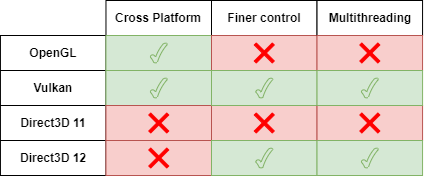
\includegraphics[width=\textwidth]{images/api_comparison.png}
  \caption{Rendering API comparison}
  \label{fig:api_comparison}
\end{figure}

It shows that the Direct3D \glspl*{api} are not cross-platform and are only
created to target Microsoft-backed operating systems such as Windows and Xbox.
On the other hand, OpenGL and \gls*{vulkan} are designed according to their
specifications to run on different platforms.

\subsection{External Libraries}
The use of external libraries is vital in allowing \gls*{vmve} to be implemented
within the short timeframe allocated. Libraries provide functionality that the
application can easily incorporate without the need to implement the same
solution from scratch.

\subsubsection{Model Loading}
- Assimp, tinygltf, tinyobj
\subsubsection{User Interface}
imgui, qt, 
\subsubsection{Encryption}
crypto++, 
\subsubsection{Serialisation}
cereal, boost


\subsection{Task Management}
Task management refers to the use of tools to aid in managing tasks or issues.
Various tools are designed for this purpose however, there are two that are the most
well-known which are Trello and GitHub Projects also known as GitHub issues.

The Trello platform was developed before GitHub Projects. It also provides far
more features that can be used to better manage the project and the various
tasks that will be created throughout the development process. On the other
hand, GitHub Projects is much more integrated into the GitHub ecosystem making
it far easier to incorporate GitHub issues as tasks and also for the project
repository as a whole.

\clearpage
\section{Design} \label{design} 
The design of the project consists of selecting the specific tools discussed in
the technology review \ref{technology_review} and the architectural design
decisions for both the source code and front end of the application.

\subsection{Tools}
\subsubsection{Git/GitHub} \label{project_management}

The \gls*{vcs} that was chosen for this project was Git including the GitHub
platform \cite{gitvcs}. It's the most popular version control system as
mentioned and is the platform that I am most familiar with. Additionally, the
performance benefits that it provides over similar systems are ideal for this
type of project. Appendix section \ref{github} provides additional information
regarding the technical details of how the repository is hosted on GitHub.

\subsubsection{GitHub Projects}
Having evaluated the pros and cons of both Trello and GitHub Projects, the
decision was made to use GitHub as the platform for task management/tracking.
``posts'' are created that would track outstanding tasks including the priority,
current progress and the expected deadline. Figure \ref{fig:kanban_design} shows
a preview of the Kanban board. It consists of three main columns used to
categorise an issue including backlog, in progress and done.

When an idea for a new feature is formed or a bug within the application is
discovered a GitHub issue is created and moved to the ``Backlog'' board. This is
used to document a particular task that needs to be worked on within a desired
timeframe.

Then, once a specific issue is ready to be worked on/resolved, it's moved to the
``In Progress'' board. As the issue is being addressed, key points of discussion
are added as comments to the issue for documentation purposes and to be referred
back to within commits or merges.

Lastly, once the task has been completed, the GitHub commit that includes the
specific fix is referenced in the issue and is then finally marked as complete
by being moved to the ``Done'' board. This subsequently marks a GitHub issue as
closed.
\begin{figure}[H]
  \centering
  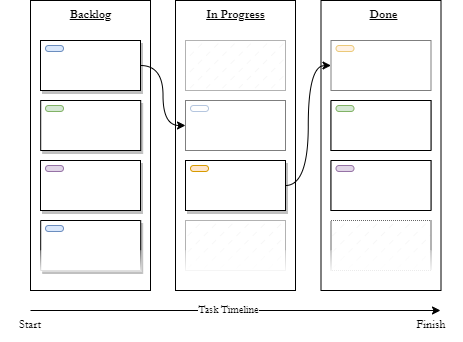
\includegraphics[width=\textwidth]{images/kanban_design.png}
  \caption{Kanban design}
  \label{fig:kanban_design}
\end{figure}

Overall, this organisation and management of tasks allow the project to meet key
sprints and deadlines and allow for issues to be resolved within a suitable
timeframe.

\subsubsection{Microsoft Visual Studio 2022} \label{development_environment}
Out of the proposed development environments, Microsoft Visual Studio 2022 was
chosen. This is primarily because of the vast amount of features and
functionality that it provides compared to the other tools. Additionally, in
conjunction with Visual Studio, Visual Studio Assist X will be used to further
improve the ease of development cite{visualstudioassistx}. This is an extension
that provides many useful features that the base \gls*{ide} does not provide
such as reliable symbol renaming, file symbol outlining and quick file
searching.

\subsubsection{RenderDoc}
As well as using software for debugging on the \gls*{cpu}, there also exists
software that allows for debugging the \gls*{gpu}. More specifically, these
tools allow for analysing per-frame data as well as detailed frame
synchronisation metrics. RenderDoc developed by Baldur Karlsson can be used to
inspect different rendering \glspl*{api} including individual frames and its
entire state \cite{renderdoc}. This ensures that you can debug specific
\gls*{gpu} related bugs such as model data, textures, rendering commands etc.

\subsubsection{AMD Radeon GPU Profiler}
Similarly to RenderDoc, AMD has its own \gls*{gpu} profiling tool called ``AMD
Radeon GPU Profiler'' \cite{rgp}. This tool is only available for AMD-supported
\glspl*{gpu} which is ideal as the hardware going to be used throughout
development meets this requirement. The tool also analyses per-frame data,
however, contains more technical and detailed metrics such as command buffers,
fences and semaphores between frames and also validates \gls*{api} usage.

% \begin{figure}[H]
%   \centering
%   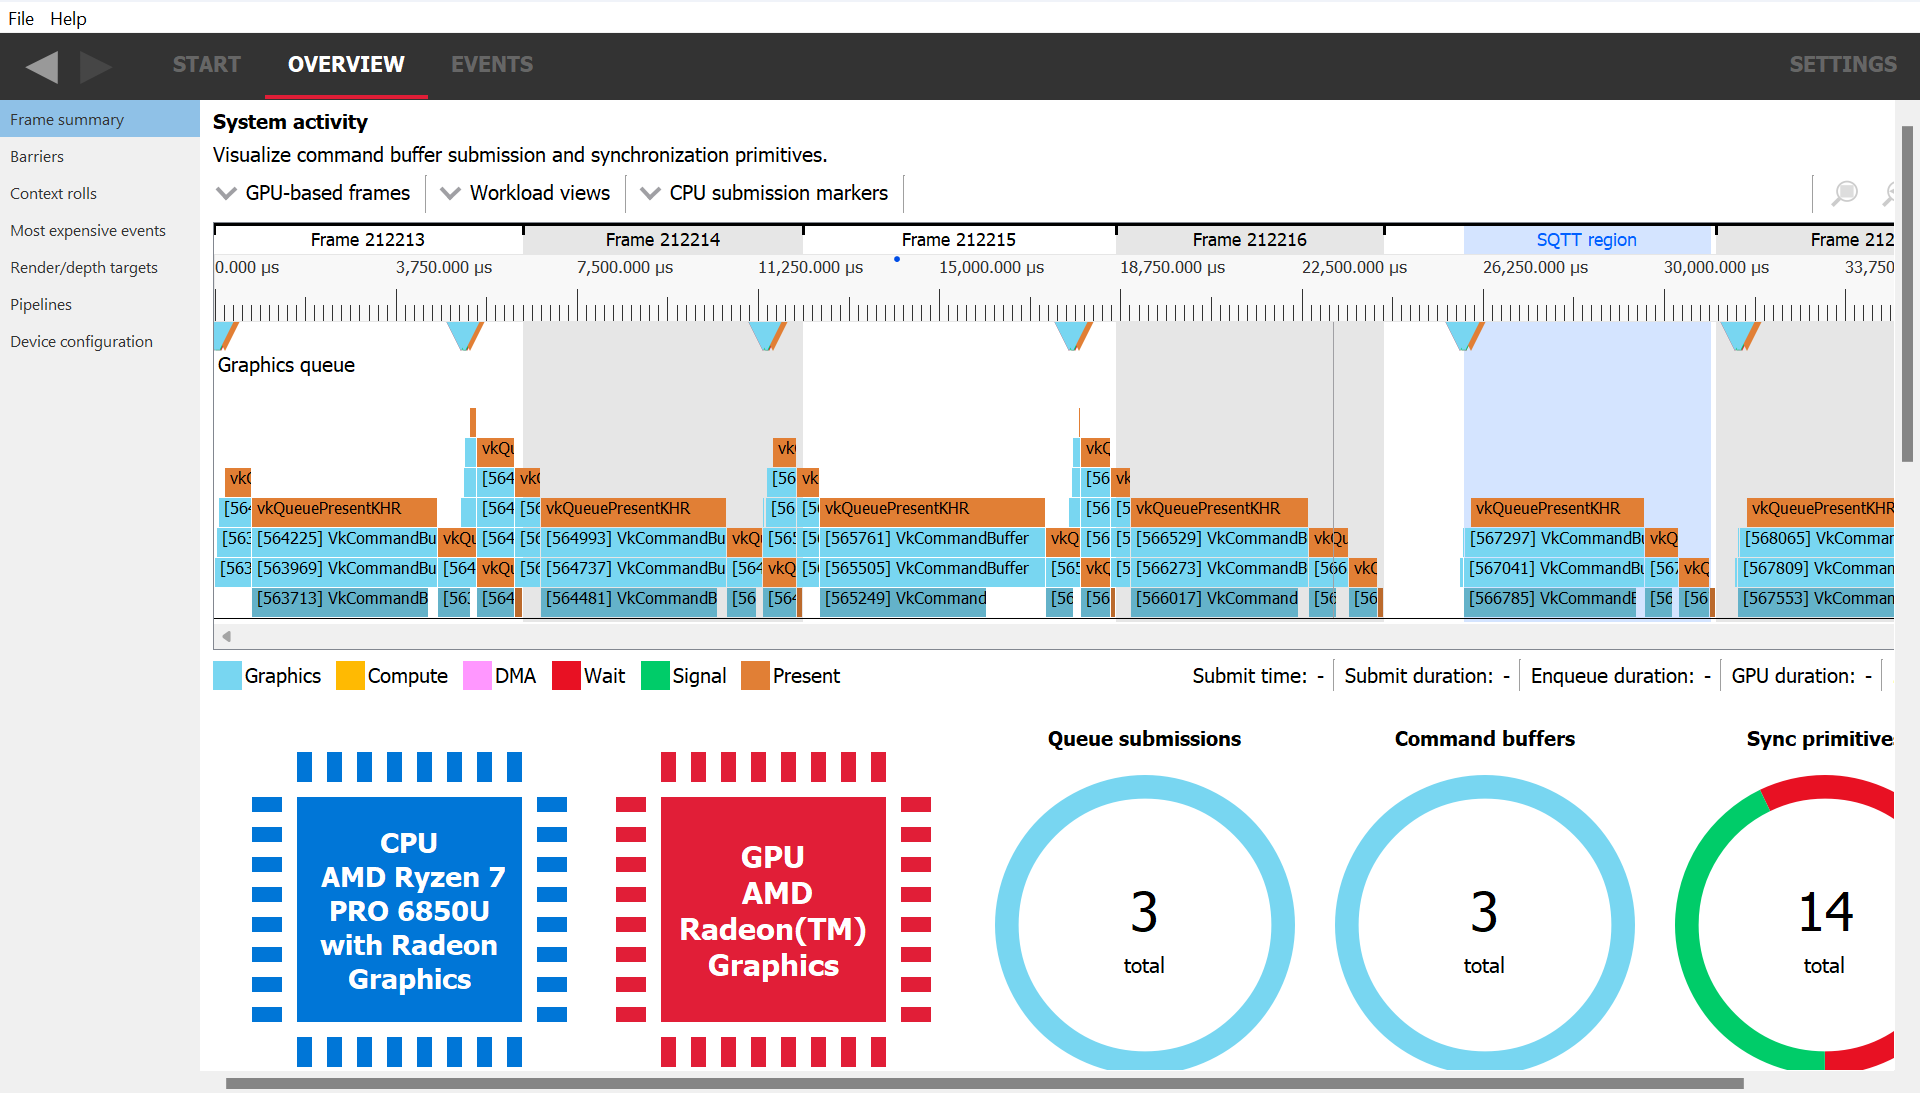
\includegraphics[width=\textwidth]{images/amd_profiler.png}
%   \caption{AMD Radeon GPU Profiler}
%   \label{fig:amd_profiler}
% \end{figure}


\subsubsection{C++ 23}
The language chosen for this project was C++ and more specifically version 23.
There were two main reasons why this specific programming language was chosen
instead of C or Rust. Firstly, it's the language that as a programmer I have the
most experience with which will significantly help during the implementation
stages of the project. Secondly, the \gls*{stl} was one of the key reasons why
C++ was chosen. It provides many prebuilt data structures, containers and
algorithms such as ``std::vector'', ``std::string'' and ``std::find'' to name a
few. Furthermore, it saves time as it eliminates the need to implement a custom
solution in the limited time frame for this project. Other language features
that confirmed the programming language was suitable included function
overloading, templates, compile-time expressions, direct memory access and
generally faster performance compared to other languages.

\subsubsection{Vulkan} \label{rendering_api}
Having evaluated the potential use of the different \glspl*{api} covered in
section \ref{rendering_api_tech_review}, it was concluded that \gls*{vulkan}
would be the most suitable rendering \gls*{api} for \gls*{vmve}. Firstly,
\gls*{vulkan} is extremely verbose as it exposes the technicalities related to
the \gls*{gpu} and requires the application to implement the basic functionality
as opposed to the underlying driver provided by major \gls*{gpu} vendors. This
reduces the complexity of the display driver and can potentially increase
performance as it no longer needs to make assumptions about the application and
the commands being issued as the entire state of the rendering pipeline is
predefined. \gls*{vulkan} was also chosen as the technology allows one to learn
and understand the complex inner workings of graphics applications and pipelines
as well as \gls*{gpu} computation. Furthermore, Figure \ref{fig:api_comparison}
shows that the \gls*{api} provides the most amount of functionality including
the ability to run on different operating systems, finer rendering control and
support for multithreading.

\begin{figure}[H]
  \centering
  
\includegraphics[width=\textwidth]{images/vulkan_logo.png}
  \caption{Vulkan logo \cite{vulkan}}
  \label{fig:vulkan_logo}
\end{figure}


\subsection{Libraries}
The application will make use of different external libraries to help aid and
speed up development as a result of the short timeframe. These libraries vary in
terms of functionality and will provide a solid foundation on which the
application can be built on top of.

\subsubsection{ImGui v1.89}
Users will need a way of interacting with \gls*{vmve} and the 3D environment at
runtime. This will be achieved through the use of a user interface in which the
user can directly manipulate the application. As mentioned earlier, \gls*{vmve}
is an application that uses the \gls*{gpu} for rendering and therefore, the UI
will have to interact with the \gls*{gpu}. To reduce the development time of
this particular aspect of the application, the decision was made to make use of
an existing library. This library is called Dear ImGui \cite{imgui}. This is an
immediate-mode user interface library that provides an \gls*{api} to render UI
elements. It's easy to use and popular which is what makes is an ideal choice.

\subsubsection{Crypto++ v8.7} \label{custom_file_format}
\gls*{vmve} will include its own model file format. This is a custom format that
will be encrypted as standard. Implementing encryption is a very complex area
that can be considered an entire project on its own. Instead, the project will
make use of a well-known encryption library known as Crypto++ \cite{cryptopp}
and the application will use version 8.7. This is a C++ library that provides
many algorithms including AES, Diffie-Hellman, GCM, RSA and much more.

\subsubsection{Cereal v1.3.2}
In addition to encrypting the model data, the custom file format will need to
store additional information such as application version and encryption type.
Therefore, \gls*{vmve} must be able to serialise the data when saving to disk as
well as deserialise when loading a ``.vmve'' model. To achieve this, the cereal
C++ library will be used \cite{cereal}. This library allows for fast and
efficient data serialisation into different formats such as compact binary
encodings, XML or JSON.

\subsubsection{Summary}
Several other external libraries were used which are shown in figure
\ref{fig:library_versions}. 

\begin{figure}[H]
  \begin{center}
    \rowcolors{2}{gray!25}{white}
    \begin{tabular}{cc}
      
      \rowcolor{gray!50}
      Assimp (Model Loading) &  v5.2.5\\
      GLM (Mathematics) &  v0.9.9.8\\
      STB (Image Loading) &  v2.27 \\
      VMA (Vulkan Memory Allocator) &  v3.1.0 \\
      VOLK (Vulkan Function Loader) & v1.3215 \\
      ENTT (Entity Component System) & v3.11 \\
    \end{tabular}
  \end{center}
  \caption{Additional library versions}
  \label{fig:library_versions}
  \end{figure}

\subsection{Branding}
The branding i.e. the look of the application was an important factor during the
design as it will be presented to users and can directly influence the user
experience. Additionally, Being recognisable results in an increase in brand
recognition that may also increase user traffic as found in a 2013 paper titled
\textit{The role of logos in building brand awareness and performance:
implications for entrepreneurs} \cite{girard2013role}.

\subsubsection{Project Name}
VMVE stands for ``Vulkan Model Viewer and Exporter''. The name is made up of two
parts. The first is ``Vulkan'' the other is ``Model Viewer and Exporter''. The
rendering \gls*{api} used to render 3D digital assets is \gls*{vulkan} and hence
the first part of the name. The second part is because the application will
include functionality such as importing and exporting models into a custom file
format as mentioned in section \ref{custom_file_format}. The combination of
these two allows a user to have a basic understanding of what the application
does without having used it before which is also known as a descriptive logo.

\subsubsection{Logo}
There are two versions of the \gls*{vmve} logo that was designed and intended to
be used in different scenarios. The first is the complete logo as seen below in
figure \ref{fig:project_logo_large} which is referred to as the ``large logo''.
It contains the icon and the name of the application to the right of that.
\begin{figure}[H]
  \centering
  
\includegraphics[width=\textwidth]{images/project_logo.png}
  \caption{VMVE Large Logo}
  \label{fig:project_logo_large}
\end{figure}
This is to be used on the \gls*{vmve} website as well as documentation pages
providing consistent branding across different mediums.

The second version is designed to be minimal and therefore, only consists of the
icon. This is intended to be mainly used throughout the application and in
locations where there is a minimal amount of space such as the Windows taskbar.
\begin{figure}[H]
  \centering
  
\includegraphics[width=0.25\textwidth]{images/project_icon.png}
  \caption{\gls*{vmve} Small Logo}
  \label{fig:project_logo_small}
\end{figure}


\subsection{Project Architecture}

\subsubsection{Development Life Cycle}
Agile will be the development life cycle of choice through the project's
development. This is a software development methodology which is an iterative
process occurs for key stages of a project. This allows for continuous
designing, implementation and evaluation that ensures requirements are being
adhered to.

\begin{figure}[H]
  \centering
  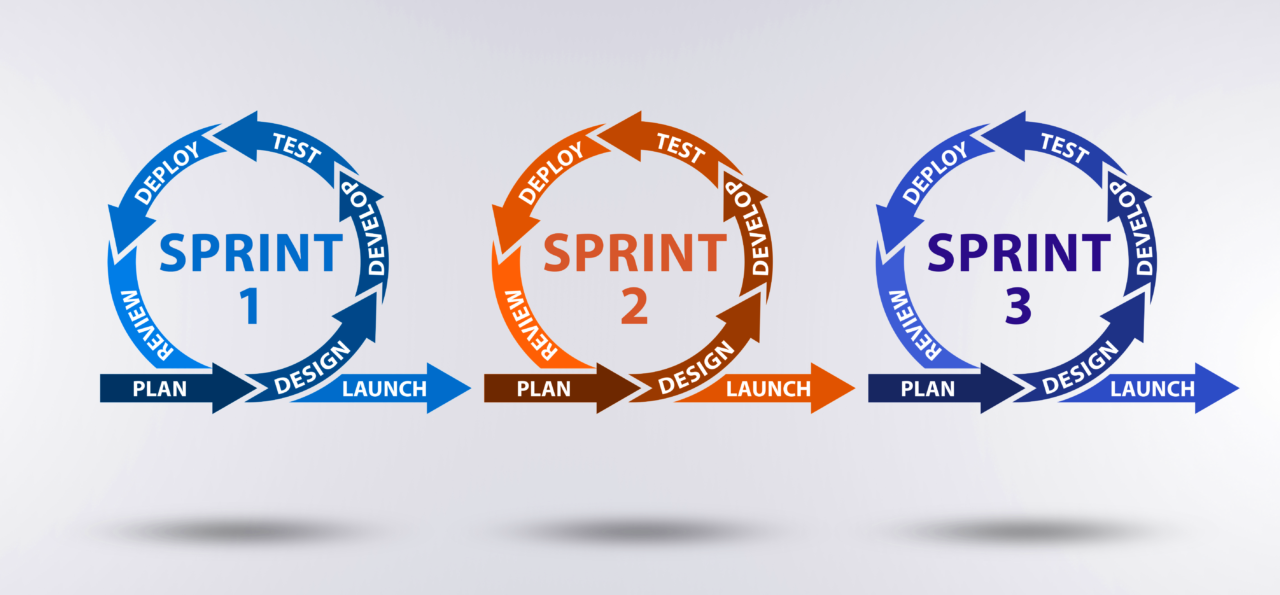
\includegraphics[width=\textwidth]{images/development_life_cycle.png}
  \caption{Agile Development Life Cycle \cite{agile}}
  \label{fig:development_life_cycle}
\end{figure}

\subsubsection{Version Control}
As the only developer for this final-year project, the design and architecture
of the \gls*{vcs} will remain as simple as possible while still providing the
core requirements. Figure \ref{fig:brancharch} shows the proposed \gls*{vcs}
architecture and includes two branches named ``main'' and ``develop''. Develop
branch will be the primary branch used throughout the implementation stages. In
other words, when changes occur throughout the source code, all commits will be
published to the development branch.

On the other hand, ``Main'' will be used as a stable branch that is only updated
for each official release. This would occur for each project milestone such that
for ``Sprint 1'' a pull request will be made from develop to main and this will
be tagged as v0.0.1 and likewise ``Sprint 2'' will be tagged as v0.0.2.

\begin{figure}[H]
  \centering
  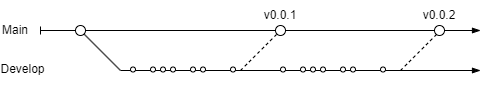
\includegraphics[width=\textwidth]{images/current_branch_design.png}
  \caption{Git branch design}
  \label{fig:brancharch}
\end{figure}

This architecture ensures that as the sole developer of the project, changes can
be made consistently while ensuring that users are provided stable versions of
the application.

\subsubsection{Source Code}
The source code for the application and overall architecture are to adhere to
the C++ core guidelines \cite{cpp-guidelines} to ensure that the project follows
best practices. Section
\href{http://isocpp.github.io/CppCoreGuidelines/CppCoreGuidelines#nl10-prefer-underscore_style-names}{NL.10}
of the core guidelines recommend using the snake case style as it follows the
standard libraries naming convention. Since the project has no existing code
base and therefore, no existing convention to follow, the project will make use
of the underscore style for types, functions and variables. 

Additionally, section
\href{https://isocpp.github.io/CppCoreGuidelines/CppCoreGuidelines#nl17-use-kr-derived-layout}{NL.17}
states that the use of the ``K\&R''  indentation style \cite{indentation} should
be used as it preserves vertical space whilst maintaining readability. In other
words, reducing vertical line height for code blocks such as ``if, else, while
and for'' allowing for more lines of code to be visible at any given point
whilst allowing for a more distinct separation of structures and functions.

The combination of these two specific conventions regarding source code style
can be seen in figure \ref{fig:convention}.

\begin{figure}[H]
\centering
\begin{lstlisting}[language=C++]
  struct foo
  {
      int a;
  };

  void bar(int a)
  {
      if (a) {
          printf("This is a example.\n");
      } else {
          printf("This is another example.\n");
      }
  }
\end{lstlisting}
\caption{Source code convention}
\label{fig:convention}
\end{figure}

\gls*{vmve} will also be developed in a functional style and by using ``structs``
instead of an object-oriented one with ``classes''. This is primarily related to
the ease of use in terms of development since data can be more easily accessed
and manipulated. Furthermore, this will eliminate the need for getter and setter
functions that needlessly take up source code space and is redundant when member
variables are accessible.

\subsubsection{Architecture}
\gls*{vmve} will be a combination of two projects. The ``Engine'' project also
known as the core of \gls*{vmve} will contain the fundamental implementation
details. This includes the Window, Renderer, UI and Audio. This project will be
distributed as a library file (.lib) that other projects can import for specific
use cases. The ``VMVE'' project will include the ``Engine'' project by importing
the library (.lib file). A high-level overview of the project architecture can
be seen in figure \ref{fig:projarch}. Furthermore, by making this distinction
between the core and \gls*{vmve}, it will allow for the same sets of tools and
technologies to be used in the future for other similar projects.

\begin{figure}[H]
  \centering
  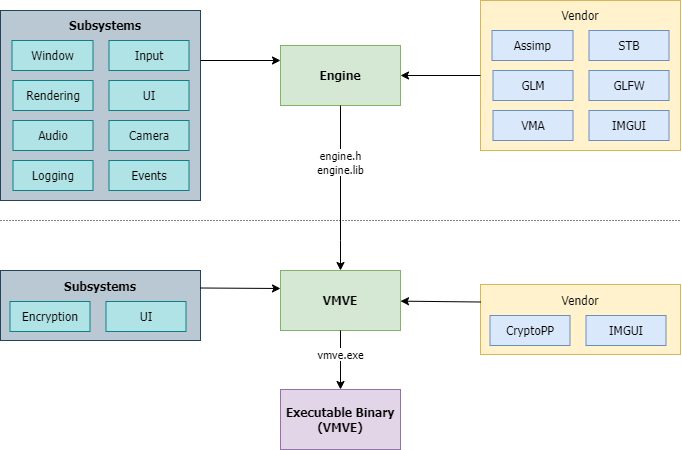
\includegraphics[width=\textwidth]{images/project_architecture.png}
  \caption{Project Architecture}
  \label{fig:projarch}
\end{figure}

\subsubsection{Platform Architecture}
The application will be developed to take advantage of the 64-bit platform. This
would allow for the application to go beyond the 4GB limit posed by 32bit
programs. In addition to this, 64-bit provides better performance and security
as a result of the larger address space.

\subsubsection{Renderer Architecture}
As mentioned in section \ref{rendering_api}. Vulkan will be the rendering API of
choice for \gls*{vmve}. The API is extremely verbose giving the programmer the
flexibility to control every aspect of the GPU. When interacting with Vulkan
throughout the engine a certain degree of encapsulation is necessary to reduce
the amount of effort required to implement functionality as a result of
\glspl*{vulkan} verbose API.

Therefore, the renderer must be designed so that flexibility is maintained
whilst simplifying the \gls{api}. Figure \ref{fig:rendererarch} shows the
proposed renderer architecture which makes distinctive boundaries and
encapsulates key sub-systems.

\begin{figure}[H]
  \centering
  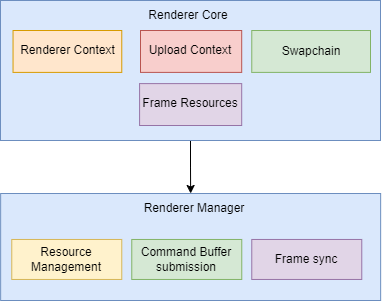
\includegraphics[width=\textwidth]{images/renderer_architecture.png}
  \caption{Renderer Architecture}
  \label{fig:rendererarch}
\end{figure}

\subsection{User Interface}
Designing the user interface was the next step as part of the design stage of
the project. Figure \ref{fig:ui_design} shows the initial user interface
wireframe that includes four main elements titled ``Global Controls'', ``Logs'',
``Model Controls'' and ``Main Viewport''. Each of these UI elements is located
in their respective windows which are designed in such a way that common
controls are grouped and located appropriately if not within the same panel.

\begin{figure}[H]
  \centering
  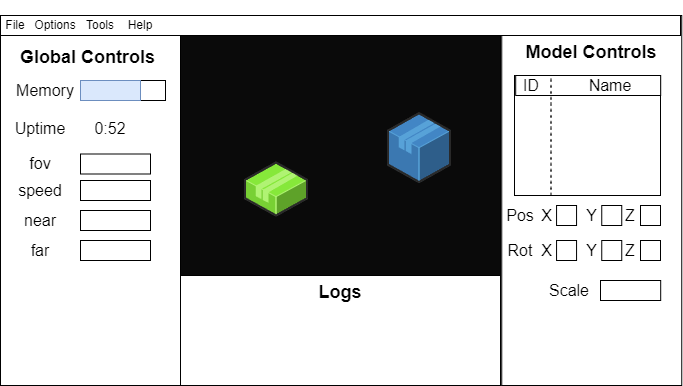
\includegraphics[width=\textwidth]{images/ui_design.png}
  \caption{UI Design}
  \label{fig:ui_design}
\end{figure}

The purpose of the user interface is to provide an easy-to-use platform for
interacting with \gls*{vmve} and more specifically the main viewport located in
the center of the application.

\subsubsection{Main Viewport}
The main viewport is located in the center of the window and is the main window
of the user interface. The main viewport renders and displays the virtual
environment.

\subsubsection{Global Panel}
Located on the left side of the application, the global controls panel will
contain user interface elements that apply globally such as general application
information and camera controls.

\subsubsection{Model/Entity Panel}
The right side panel called model controls will display model and entity
specific information and will be the primary control surface for interacting
with objects in the virtual environment.


\subsubsection{Logs Panel}
The logs panel is designed to contain all internal messages that the application
prints out. These messages will then be displayed within the logs panel. Each
log message will be categorised as either log, warning or error. Depending on
which log type the message is, it will be shown in a different color such as
white, orange or red respectively.

This is designed so that the user will have a clear understanding of the internal state
of the application.

\subsection{Custom File Format and Encryption}

\subsubsection{File format}
\gls*{vmve} will include a custom file format that allows for model data to be
encrypted for security purposes. Figure \ref{fig:vmve_file_structure} shows the
proposed internal structure of the file. The internal structure is split into
two main sections. The header contains key pieces of information that help the
application determine how and if the main data should be decrypted.

\begin{description}
  \item[Version] indicates which version of \gls*{vmve} was used to encrypt the
  file. At the moment, this is to be purely informational however, in future
  versions, this can be used for reporting compatibility issues and also,
  allowing for encrypted files to be updated to newer file layouts.
  \item[Mode] is the encryption algorithm used (e.g AES, DH) and is what will
  allow the application to know which decryption algorithm needs to be used.
  \item[Encrypted Keys] is used for validating the input key and initialisation
  vector. If these match then the application will then decrypt and load the data.
\end{description}

The second item in the \gls*{vmve} header is the encryption mode. This allows for
\gls*{vmve} to know which algorithm must be used to decrypt the data.

The remaining section of the file consists of the encrypted data which includes
the raw model data.

\begin{figure}[H]
  \centering
  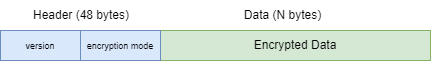
\includegraphics[width=\textwidth]{images/vmve_file_structure.png}
  \caption{VMVE File internal structure}
  \label{fig:vmve_file_structure}
\end{figure}


\subsubsection{Encryption and Decryption}
When dealing with encryption there are two primary stages, encrypting and
decrypting. The term ``encryption'' means taking some data and running it
through an algorithm making the data unreadable. ``Decryption'' is the opposite
of that which takes the unreadable data and turns it back to the original data.

Designing such a system requires careful consideration and extra care to ensure
that the data being managed is not negatively affected such as information being
lost when converting from one stage to another.

The primary encryption algorithm that will be used is AES and the key length can
be two different values (128 or 256 bits) that the user will choose based on the
level of security they want for their assets.

Figure \ref{fig:load_model_flowchart} shows a flowchart describing the general
process of how a model will be loaded into \gls*{vmve}.

\begin{figure}[H]
  \centering
  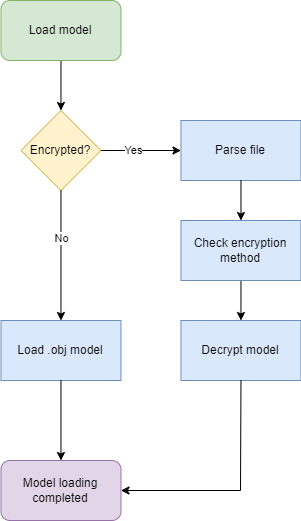
\includegraphics[width=0.5\textwidth]{images/load_model_flowchart.png}
  \caption{Load model flowchart}
  \label{fig:load_model_flowchart}
\end{figure}

Likewise encrypting a model will consist of three main stages which are loading, encrypting
and exporting as show in figure \ref{fig:export_model_flowchart}.
\begin{figure}[H]
  \centering
  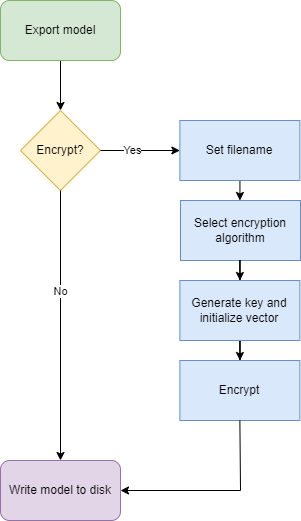
\includegraphics[width=0.5\textwidth]{images/export_model_flowchart.png}
  \caption{Export model flowchart}
  \label{fig:export_model_flowchart}
\end{figure}

\clearpage
\section{Implementation} \label{implementation}

This section of the report presents the technical implementation details of
\gls*{vmve} and is structured in order of initialisation i.e starting at the
core of the application and discussing each subsequent system. 

\begin{figure}[H]
  \centering
  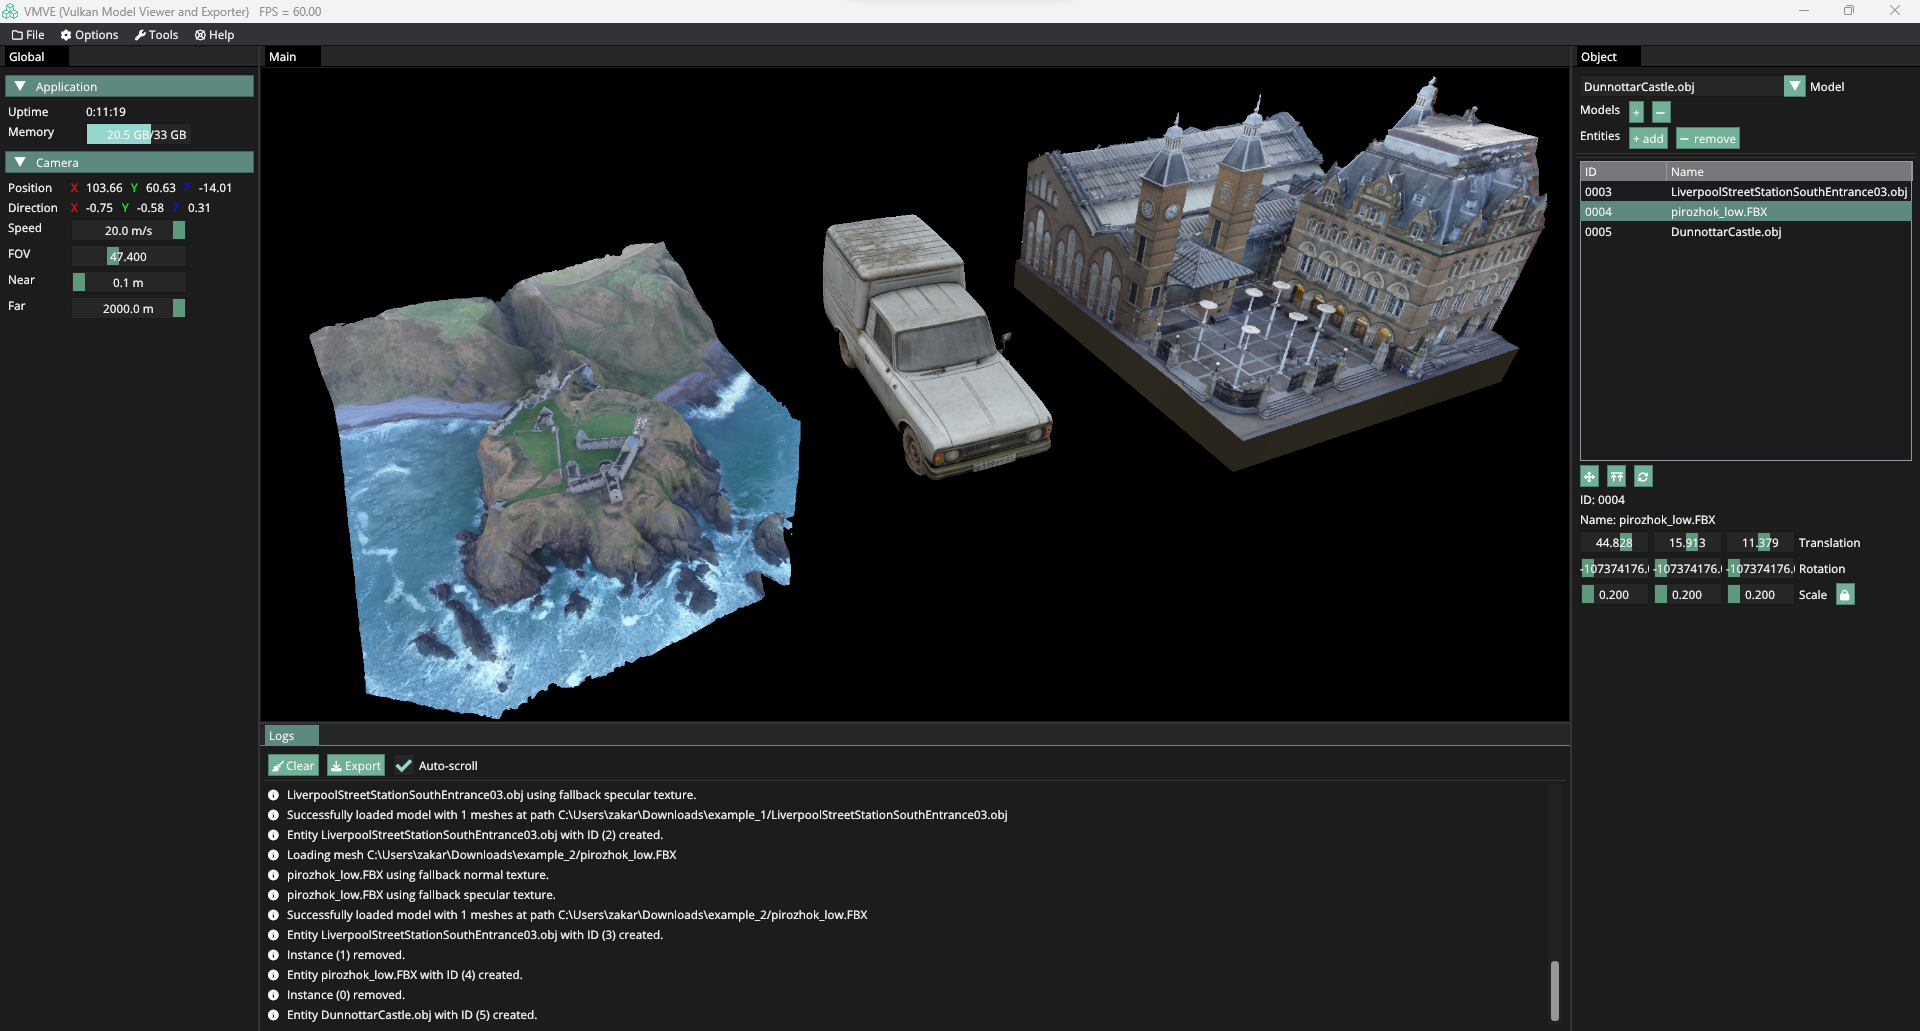
\includegraphics[width=\textwidth]{images/ui_implementation.png}
  \caption{UI implementation}
  \label{fig:user_interface}
\end{figure}

% \begin{figure}[H]
%   \centering
%   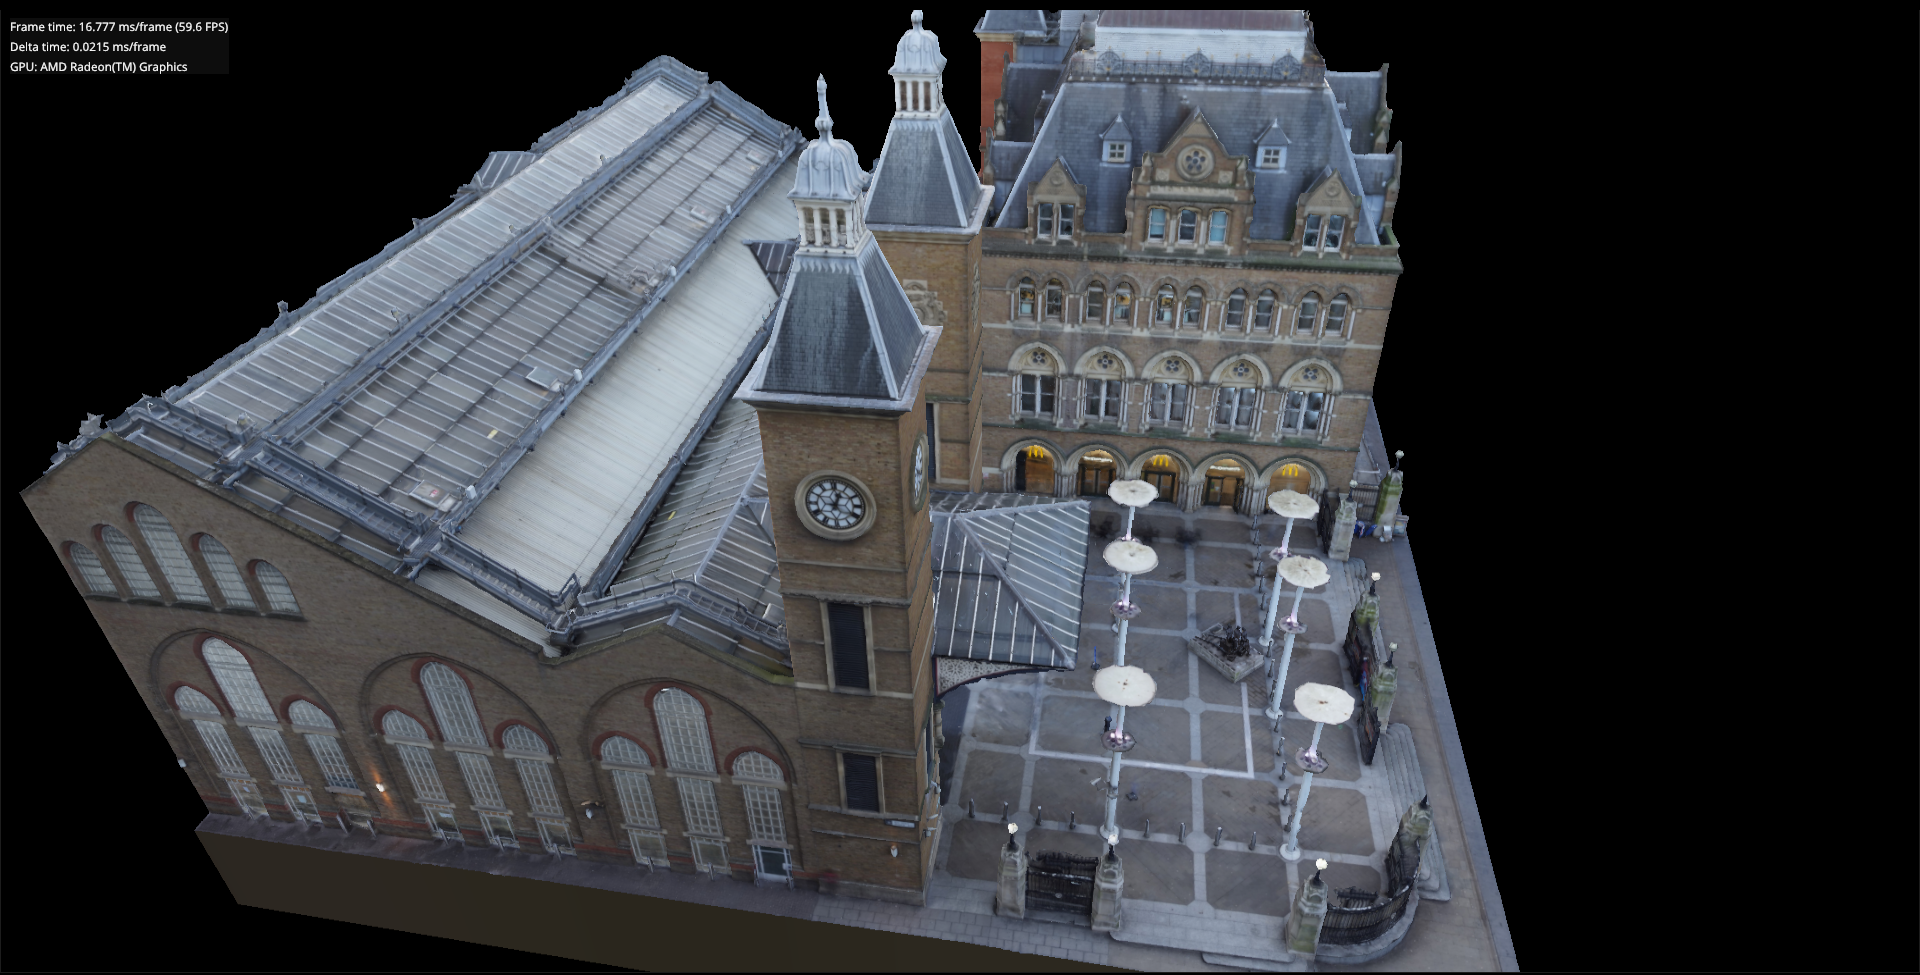
\includegraphics[width=\textwidth]{images/rendering.png}
%   \caption{Liverpool Street Station renderer model}
%   \label{fig:renderer}
% \end{figure}


\subsection{Overview}
Figure \ref{fig:overview_pseudo_code} shows the general overview of the
application and the various stages that occur during initialisation, runtime and
shutting down. The application is a complex system that consists of various
subsystems that work together.


\begin{figure}[H]
\centering
\begin{lstlisting}[language=C++]

int main()
{
  // begin application initialisation
  create_window(width, height, name);
  create_renderer();
  create_audio();
  create_ui();

  // set default configuration options
  create_camera();
  
  // begin application rendering
  while (running)
  {
    update_renderer();

    render_geometry();
    render_ui();

    update_window();
  }

  // shutdown application
  destroy_ui();
  destroy_audio();
  destroy_renderer();
  destroy_window();

  return 0;
}
\end{lstlisting}
\caption{Implementation overview pseudo code}
\label{fig:overview_pseudo_code}
\end{figure}

  

\subsection{Window System}
The first system within \gls*{vmve} that gets initialised is the window. This system is
responsible for creating a desktop window based on a series of configuration
options specified at the start of the application. These options include the
window width, height and name. Internally, \gls*{vmve} uses the lightweight GLFW
library to handle window creation. The purpose of this library is to provide an
API which is cross-platform and allows applications to easily create windows on
different operating systems. 

Under the hood, on Windows, GLFW uses the Win32 API provided by Microsoft.

In addition to the window creation, various function callbacks are created
which allows \gls*{vmve} to handle specific events such as window resizing, input,
cursor position etc.

\subsection{Rendering System}
The implementation of the rendering system was one of the key areas worked on
throughout the project. This system is responsible for communicating with the
\gls*{gpu} and rendering objects onto the screen. As discussed in the
\ref{technology_review}, Vulkan was the renderer API of choice. 

    

\subsubsection{Renderer Context}
The first step in creating the renderer is initialising an object called
``vk\_context''. This object is created within the application that groups
Vulkan handles that is responsible for initialising resources. In other words,
the ``vk\_context'' structure is used to allocate \gls*{gpu} resources. The
handles within the context structure can be seen in the code snippet below and a
diagram can be seen in figure \ref{fig:rendererarch}.

\begin{lstlisting}[language=C++]
struct vk_context
{
  VkInstance         // Initialises Vulkan library
  VkPhysicalDevice   // Handle to physical hardware
  VkDevice           // Logical handle to physical hardware
  VkQueue            // Graphics queue
  VkQueue            // Presentation queue
  VmaAllocator       // VMA memory allocator
};
\end{lstlisting}

The initialisation of the renderer context can be broken down into several
stages. The first of these states acquires the function pointers into the Vulkan
loader which contains the implementation details for the \gls*{gpu} driver. This
is achieved by statically linking a ``stub'' library file into the executable.
However, as discussed in a blog post by Arseny Kapoulkine titled
\textit{``Reducing Vulkan\textsuperscript{\textregistered} API call overhead''}
\cite{volk}, he finds that this method has some overhead due to how function
calls are dispatched. To reduce this overhead, a meta-loader called Volk is used
which contains pointers to the real implementation and is dynamically loaded at
runtime.

The next step is acquiring a \gls*{gpu} with a specific set of requirements that
can be used for rendering. This step involves querying all available \glspl*{gpu}
their names, hardware capabilities as well as if it supports basic screen
rendering.

\subsubsection{Swapchain}
A swapchain is a series of images also known as framebuffers used by
\gls*{vulkan} that allocates a region of memory that stores frame data i.e pixel
colors. As the name suggests, a ``swapchain'' is a chain of these images. The
most common number of images is two or three which is called
``double-buffering'' and ``triple-buffering'' respectively. The renderer within
\gls*{vmve} is configured to use two images, one for the front buffer that is shown
on a monitor and a back buffer that is used for rendering.

In addition to buffers, a swapchain is also responsible for handling vertical
refresh rate also known as vsync. This is the rate at which new images are
rendered and then presented on a user's screen. There are two main types of
vsync modes used within \gls*{vulkan} which are
\lstinline{VK_PRESENT_MODE_FIFO_KHR} and
\lstinline{VK_PRESENT_MODE_IMMEDIATE_KHR}. The ``fifo'' mode indicates to the 
swapchain and subsequently, the presentation engine that images are to wait 
for the monitor's refresh rate before being present whereas ``immediate'' simply
renders images as fast as possible.

\begin{figure}[H]
  \centering
  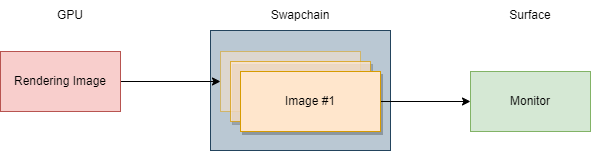
\includegraphics[width=\textwidth]{images/swapchain.png}
  \caption{Swapchain}
  \label{fig:swapchain}
\end{figure}

\gls*{vmve} uses the ``fifo'' presentation mode as it conserves hardware
resources as new images will not be rendered needlessly. Also, this mode ensures
that no screen tearing occurs between refresh rates. Figure \ref{fig:frame_sync}
shows a detailed image regarding the presentation engine and frame
synchronisation.

\subsubsection{Frame synchronisation}
Once the swapchain along with its framebuffers has been fully initialised, the
renderer can now start creating the necessary resources required for frame
synchronisation. Vulkan has two concepts that relate to synchronisation which
are VkFence and VkSemaphore.

\begin{figure}[H]
  \centering
  \begin{lstlisting}[language=C++]
    struct vk_frame
    {
        VkFence submit_fence;

        VkSemaphore image_ready;
        VkSemaphore image_complete;
    };
  \end{lstlisting}
  \caption{Frame sync structure}
  \label{fig:vk_fence}
\end{figure}

The \gls*{vulkan} 1.3.246 specification states that  ``\lstinline{VkFence} is a
synchronisation primitive that can be used between queue submissions and the
host''
[\href{https://registry.khronos.org/vulkan/specs/1.3-extensions/man/html/VkFence.html}{7.3
Fences}] \cite{vulkan-spec}. In other words, a fence can be signaled on the
\gls*{cpu} to indicate in this case, when a new image from the presentation
engine has been acquired via the \lstinline{vkAcquireNextImageKHR} function
call.

Similarly, ``\lstinline{VkSemaphore} is a synchronisation primitive that can be
used between queue operations''
[\href{https://registry.khronos.org/vulkan/specs/1.3-extensions/man/html/VkSemaphore.html}{7.4
Semaphores}] \cite{vulkan-spec}. For the application, this means that rendering
operations can occur simultaneously for multiple frames while ensuring that
frames ``in-flight'' are not interrupted.


\begin{figure}[H]
  \centering
  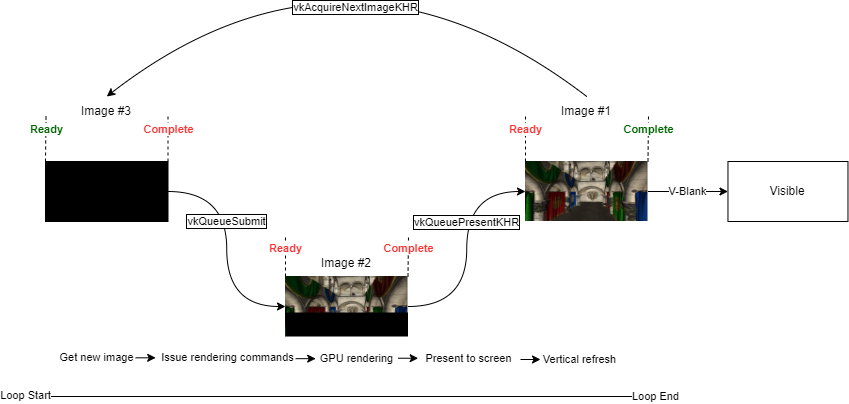
\includegraphics[width=\textwidth]{images/frame_sync.png}
  \caption{Frame Synchronisation}
  \label{fig:frame_sync}
\end{figure}

\subsubsection{Deferred Rendering Pipeline}
The next rendering feature that was implemented was a deferred rendering
pipeline. During rendering, there are two main passes. The first pass renders
the raw geometry data and performs MVP translation (section \ref{camera}). For
each rendered frame a total of five framebuffers are filled with different types of
information including colors, world positions, normals, depth and specular.

Then the second pass reads the data from the five framebuffers and performs the
lighting calculations. This is a common technique in rendering applications that
significantly improve performance when large numbers of light sources are
present compared to forward rendering. This is because deferred rendering defers
all lighting calculations to the final pass and only needs to perform those
calculations once. However, for forward rendering, this needs to occur for each
object in the scene resulting in poorer performance.

\begin{figure}[H]
  \centering
  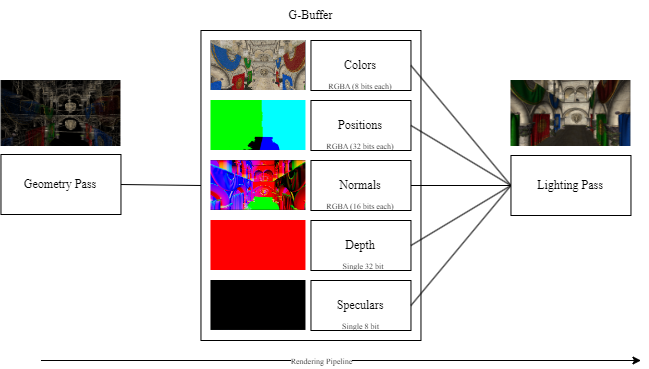
\includegraphics[width=\textwidth]{images/g_buffer.png}
  \caption{G-Buffer Pipeline}
  \label{fig:g_buffer}
\end{figure}



\subsubsection{Dynamic Uniform Buffers}
Uniform buffers are regions of memory located in \gls*{vram} on the \gls*{gpu}.
This memory can be accessed by shaders when creating a frame. These buffers can
contain any sort of data including camera information, light properties, object
transformations etc.

\gls*{vmve} makes use of two dynamic uniform buffers one for the camera
projection and the other for scene information such as lights. A dynamic buffer
is a buffer that is large enough to store per-frame data and each frame of data
can be accessed using an offset into the buffer and the current frame index.
Figure \ref{fig:dynamic_uniform_buffer} shows the internal structure of a dynamic
uniform buffer that stores three sub-regions of memory in a triple-buffered
frame setup.

\begin{figure}[H]
  \centering
  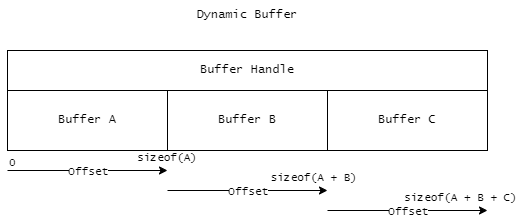
\includegraphics[width=\textwidth]{images/dynamic_buffer.png}
  \caption{Dynamic Uniform Buffer}
  \label{fig:dynamic_uniform_buffer}
\end{figure}

The use of dynamic uniform buffers provides several benefits compared to using a
unique buffer handle for each frame.

\subsubsection{Texture Mipmapping}
\gls*{vmve} makes use of a rendering technique known as ``Texture mipmapping''.
This improves the visual fidelity by reducing if not eliminating Moire patterns
which are visual artifacts that appear when identical patterns/textures are
transformed on the screen \cite{moire_pattern}.

\begin{figure}[H]
  \centering
  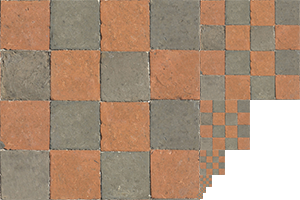
\includegraphics[width=\textwidth]{images/mipmaps.png}
  \caption{Texture mipmapping}
  \label{fig:texture_mipmapping} \cite{texture_mipmaps}
\end{figure}


Using \gls*{vulkan}, this is implemented by taking the originally loaded texture
and continuously halving it on both the width and height so that the subsequent texture is
a quarter of the previous size. This is performed using the following equation provided by
``Sascha Willems''.
\begin{equation}
  m = \lfloor \log_2(\max(w, h)) \rfloor + 1
\end{equation}
where \(m\) is the number of mipmap levels, \(w\) and \(h\) are the width and
height of the source texture respectively. For each texture mipmap created the
size of the texture becomes exponentially smaller.

In the source code, it looks like this:
\begin{figure}[H]
  \centering
  \begin{lstlisting}[language=C++]
    const auto mip_levels = static_cast<uint32_t>(std::floor(std::log2(std::max(width, height)))) + 1;
  \end{lstlisting}
  \caption{Mipmapping equation}
  \label{fig:mipmapping_equation}
\end{figure}

\subsubsection{Models}
In the context of the rendering system, a ``model'' is a structure that
represents a 3D geometry object. This could be as simple as a cube or as complex
as an entire scene. The data structure contains several key pieces of
information such as geometry data and textures. 

Complex models are not singular pieces of geometry. Instead, artists combine
multiple smaller objects to form the final model. These smaller parts are known
as ``Meshes'' within the application. Each mesh has its own vertex and index
buffers stored on \gls*{gpu} that describe to \gls*{vulkan} how the piece of
geometry is to be interpreted.

Figure \ref{fig:model} shows the internal structure of an example model which
has been loaded into \gls*{vmve}.
\begin{figure}[H]
  \centering
  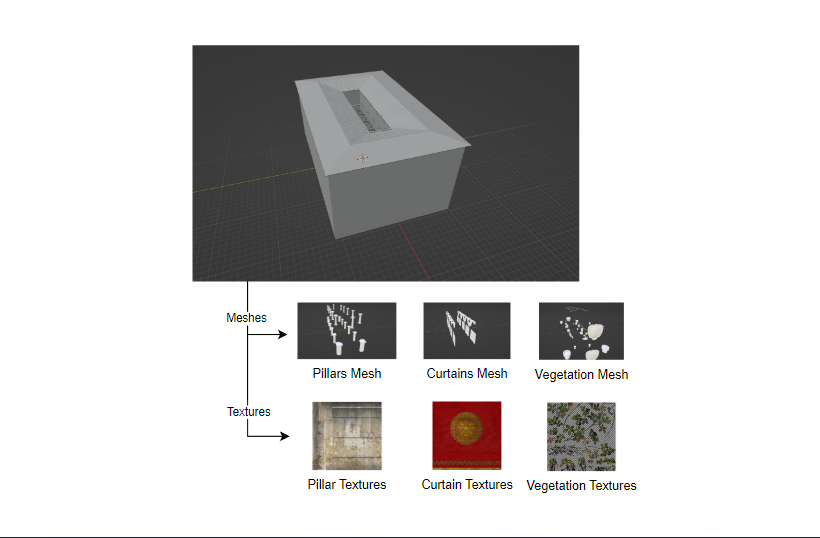
\includegraphics[width=\textwidth]{images/model.png}
  \caption{Model Structure}
  \label{fig:model}
\end{figure}

When a user loads a model, the model is appended to a continuous array
(\lstinline{std::vector<Model> models;}) which is iterated over each frame in
order to render all the models on the screen.

\subsubsection{Entities}
An entity represents an instance of the model in the virtual environment. There
can be many different entities using the same model. An example of this can be
seen in figure \ref{fig:entities} which shows four entities using the same
backpack model.

This is achieved by storing a model index that indicates which model the entity
refers to within the contiguous array of models. Secondly, an entity contains a
transformation matrix that positions the entity in the world. A more in-depth
explanation of the model matrix can be found in section \ref{camera}.

\begin{figure}[H]
  \centering
  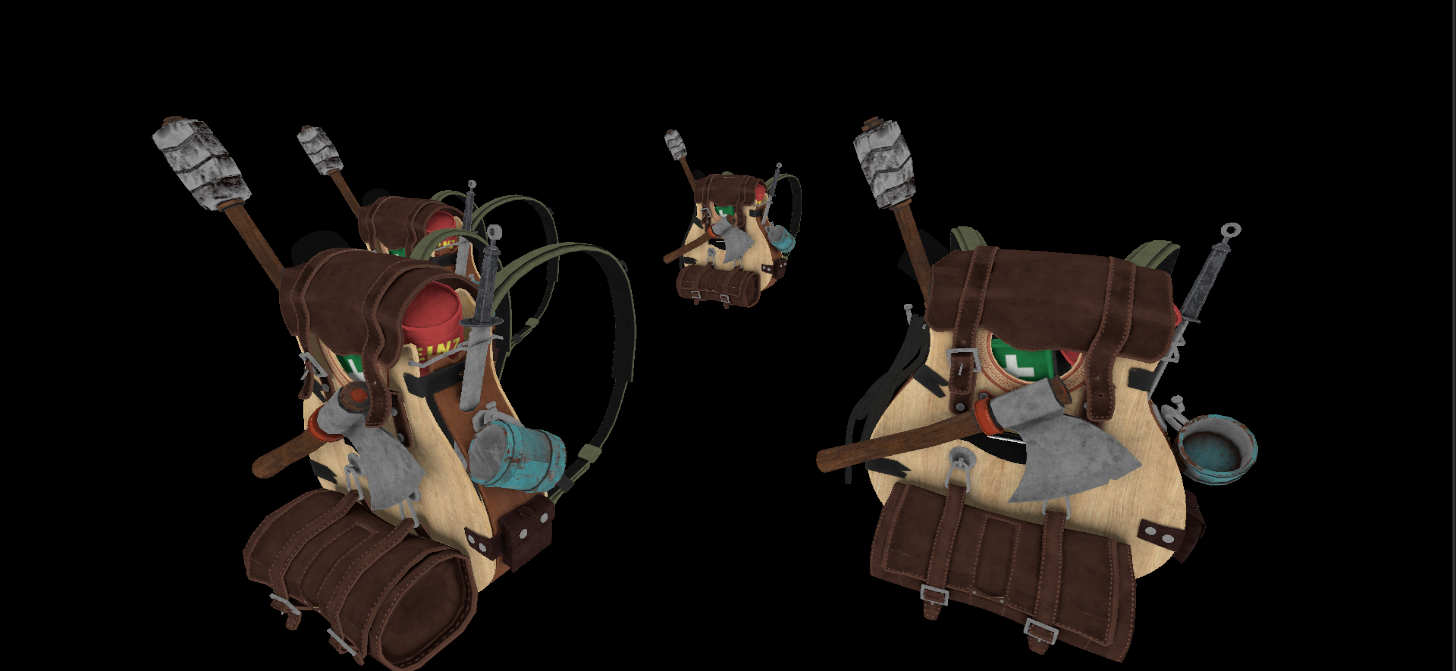
\includegraphics[width=\textwidth]{images/entities.png}
  \caption{Multiple entities in virtual environment}
  \label{fig:entities}
\end{figure}

\subsubsection{Camera} \label{camera}
3D geometry data must be transformed through a series of mathematical
calculations that will take vertex points from a 3D ``world'' and then convert
them onto a 2D image for it to then be displayed on a monitor. This
transformation is known as perspective projection \cite{3d_projection} and is
accomplished by computing several intermediate coordinate spaces as seen in
figure \ref{fig:mvp_projection}.

\begin{figure}[H]
  \centering
  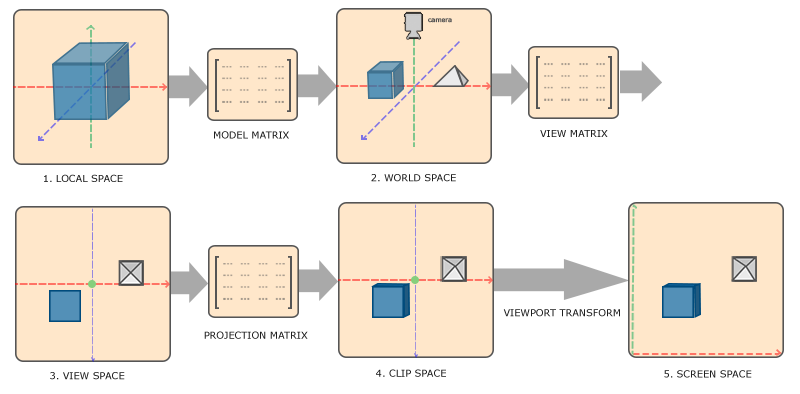
\includegraphics[width=\textwidth]{images/mvp.png}
  \caption{MVP Transformation \cite{coordinate_systems}}
  \label{fig:mvp_transformation} 
\end{figure}

Geometric data is first created within a local coordinate space. This ``space''
is positions relative to the object. In other words, the model data imported by
\gls*{vmve} will be in this local coordinate system often created by a 3D modeling
program such as Blender or 3DSMax.

The next step is to convert these local coordinates to ``world'' space. This is
the actual virtual environment that an object will live in. The transformation
to this space is done by constructing a 4x4 matrix and performing a combination
of translation, rotation and scaling. A pseudo-code example can be seen in
\ref{fig:local_to_world}.

\begin{figure}[H]
  \centering
  \begin{lstlisting}[language=C++]
    mat4 model = mat4(1.0f);       // Identity matrix
    model = translate(position);   // Move object
    model = rotate(radians, axis); // Rotate object
    model = scale(scale);          // Scale object
  \end{lstlisting}
  \caption{Model matrix construction}
  \label{fig:local_to_world}
\end{figure}
  

The next step is transforming the world space positions to view space or also
known as camera space. This is important as how the virtual scene is displayed
depends on the properties of the camera. In the context of graphics rendering
the concept of a ``camera'' does not exist and is only really an illusion. In
reality, all points/vertex positions in the world space are transformed relative
to the ``camera''. For example, if the position of the camera along the z-axis
increases i.e. we move forward then all objects in the world will be moved
towards us. A nice visualisation of this is shown in figure
\ref{fig:camera_projection} courtesy of a blog post by Jordan Santell
\href{https://jsantell.com/model-view-projection/}{https://jsantell.com/model-view-projection/}.

\begin{figure}[H]
  \centering
  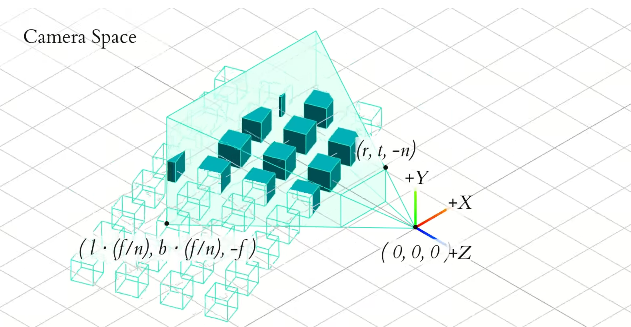
\includegraphics[width=\textwidth]{images/camera_space.png}
  \caption{Camera/view projection \cite{camera_projection}}
  \label{fig:camera_projection} 
\end{figure}

\gls*{vmve} makes use of a quaternion to perform the view projection. This is an
alternative to Euler angles and has several benefits including, preventing gimbal
lock and easier interpolation between orientations.
\begin{figure}[H]
  \centering
  \begin{lstlisting}[language=C++]
    mat4 view = lookAt(camera_position, view_direction, camera_up);
  \end{lstlisting}
  \caption{View matrix construction}
  \label{fig:world_to_view}
\end{figure}


The final step in calculating the MVP matrix is the projection which converts
points from local space to clip space. This involves projecting the points to
either a perspective or orthographic projection.
\begin{figure}[H]
  \centering
  \begin{lstlisting}[language=C++]
    mat4 proj = perspective(fovy, aspect, near, far);
  \end{lstlisting}
  \caption{Projection matrix construction}
  \label{fig:local_to_projection}
\end{figure}

With the fully constructed mvp matrix, this can now be multiplied with each
vertex position and it will display onto the screen as expected.
\begin{figure}[H]
  \centering  
  \begin{equation}
    Output = MVP \times Vertex
  \end{equation}
  \caption{MVP projection}
  \label{fig:mvp_projection}
\end{figure}

A more detailed code example can be seen in figure
\ref{fig:local_to_world_appendix} in the appendix.

\subsubsection{Lighting}
\newcommand{\intensity}{\operatorname{I}}
\newcommand{\lightdir}{\operatorname{L}}
\newcommand{\normal}{\operatorname{N}}
\newcommand{\diffuse}{\operatorname{D}}
\newcommand{\glslcolor}{\operatorname{C}}
\newcommand{\glslmax}{\operatorname{max}}

The implementation of lighting was the final rendering system that was
implemented. Lighting in Computer Graphics refers to how the virtual environment
i.e. the colors of the resulting pixels are manipulated based on certain
properties such as light, surface direction, occlusion, emissive materials and
more. The use of lighting significantly improvises the visual fidelity of the
graphics and increases the realism.

The lighting model that was implemented is called Blinn-Phong which derives from
the original Phong model was developed by Bui Tuong Phong in a paper titled
\textit{``Illumination for Computer Generated Pictures''} published in 1975
\cite{blinn}. It describes three main elements including ambient, diffuse and
specular lighting that works together to produce the final result.

\begin{description}
  \item[Ambient] Ambient is a constant value that is used instead of global illumination
    as it requires more computational resources and more complex algorithms.
    \begin{equation}
      A = G + P
    \end{equation}
  \item[Diffuse] The next step is implementing diffuse lighting. This takes into
    account the light direction $\lightdir$ and the normal $\normal$ for a
    surface at a particular pixel. The formula below calculates the intensity at
    which light reflects off of an object based on the angle off a particular
    surface.
    
    The dot product of the light direction and surface normal returns a value
    between the ranges of -1 to 1 depending on how parallel the directions are.
    If this value is equal to or less than 0 then it indicates that the light is
    behind the surface and thus, is clamped as a result of the max function
    which returns the largest value for the given two parameters.
    \begin{gather}
      \intensity = \glslmax(\vec{\lightdir} \cdot \vec{\normal}, 0) \\
    \end{gather}
    
    Having calculated the intensity value we can now simply multiply it with the
    objects' surface color as shown in the equation below.
    \begin{equation}
      \diffuse = \intensity \times \glslcolor
    \end{equation}
    
    Figure \ref{fig:diffuse} demonstrates a simple example of diffuse lighting
    and how light interacts with an object based on the various properties
    discussed. 
    \begin{figure}[H]
      \centering
      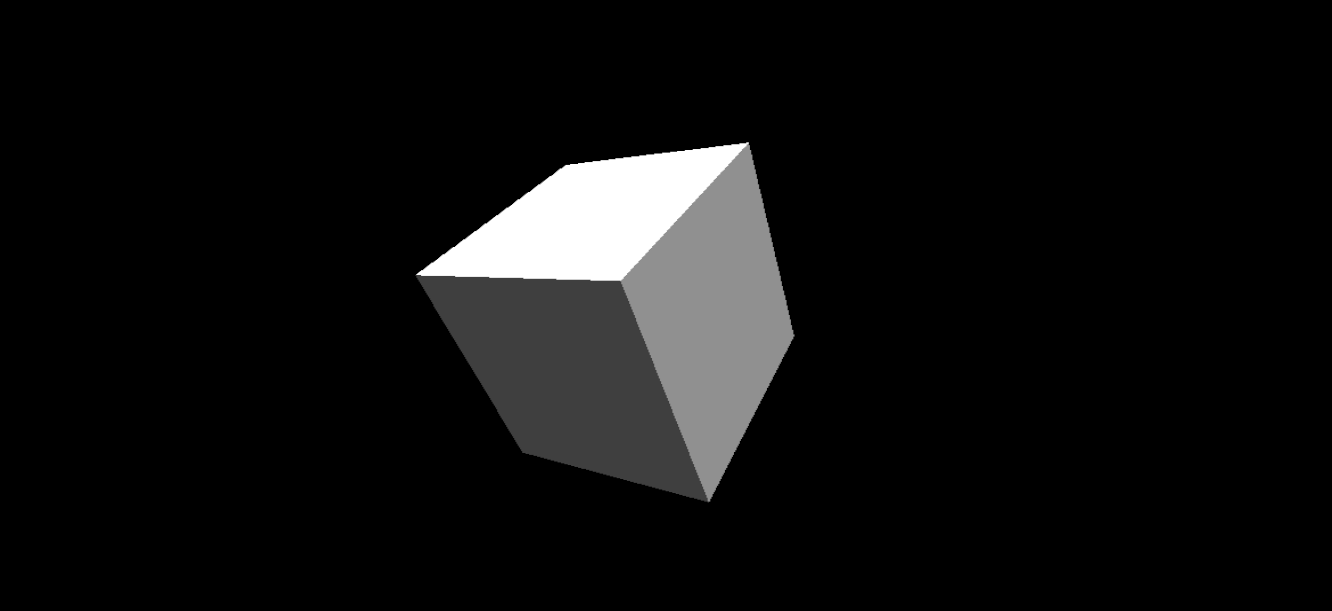
\includegraphics[width=\textwidth]{images/diffuse_lighting.png}
      \caption{Diffuse Lighting}
      \label{fig:diffuse}
    \end{figure}
  \item[Specular] The final step in the Blinn-Phong lighting model is specular.
  This effect adds highlights to certain parts of an object and is where the
  the intensity of light is strongest.
\end{description}

\subsection{User Interface}
The implementation of the user interface was the next major system. This is
the front end and how the users will be able to interact with the application.
The user interface is built on top of the Vulkan renderer.

\subsubsection{Controls}
The term ``Controls'' refers to a combination of keys also known as
``Shortcuts'' that are used to perform specific actions within the application.
Various built-in controls aim to increase productivity for the user by reducing
the amount of clicking and menu interaction for repeating tasks.

Controls are split into two categories which are Global and Viewport. Global
controls are controls that can be activated at any point. Viewport controls,
however, can only be activated whilst using the viewport i.e the camera.

This distinction for controls between different modes allows for greater context
and better usability. 

\subsubsection{Fonts and Icons}
The font used for the user interface is Open Sans which provides a simple and
easy to read font.

\gls*{vmve} also uses icons throughout the user interface and is an important
aspect in conveying key information such as the task being performed or for
additional information. The icon font used is provided by Font Awesome
\cite{font-awesome}.

Typically, data for fonts and icons are stored in a font file which ends using
extensions such as ``.ttf'' or ``.otf''. However, one of \glspl*{vmve} goals is
to be distributed as a single executable file. Therefore, we cannot depend on
external font files. Instead, data for fonts and icons are stored directly in
the application in a continuous array of bytes and are encoded in base85. A
small example of what this looks like can be seen in figure
\ref{fig:base85_font}. The full version of this is over 3000 lines long due to
the vast amount of data stored within the font.

\begin{figure}[H]
  \centering
  \begin{lstlisting}[language=C++]
    // 206 out of 201650 characters are shown

    const char open_sans_regular[201650 + 1] =
    "7])#######2Pc7('/###I),##d-LhLjKI##4%1S:`*]n8)K.v5*8_c)iZ;99=$$$$c(m]4pKdp/(RdL<snZo'oI,hLNDnx4Uu/>8Q7oo^eFb3hB4JYc'Tx-3l_wgd2Tf._r+&sAqV,-G"":F8LD=5,n]A&aA+<gXG-<iobW&>$>QJ8Z.W$jg0Fv-o^(^JJnf4T"
  \end{lstlisting}
  \caption{Base85 encoded font}
  \label{fig:base85_font}
\end{figure}

\subsubsection{Menu Bar}
The menu bar is a panel located at the top of the application and provides
global and commonly accessed tools and functionality. Each option within the 
menu bar contains various properties that allow a to toggle key settings.
\begin{figure}[H]
  \centering
  
\includegraphics[width=\textwidth]{images/menu_bar.png}
  \caption{Menu Bar}
  \label{fig:menu_bar}
\end{figure}

 
\begin{description}
  \item[File] 
    Has the main buttons for importing and exporting models. It also provides
    convenient ``Exit'' button to free all resources and terminate the
    application.
    \begin{figure}[H]
      \centering
      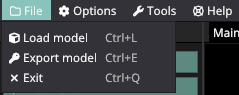
\includegraphics[width=0.5\textwidth]{images/menu_bar_file.png}
      \caption{Menu Bar File}
      \label{fig:menu_bar_file}
    \end{figure}

  \item[Options] 
    This is possibly the most frequently used item within the main menu as this
    has all the key options for the renderer and various visualisation tools.
    \begin{figure}[H]
      \centering
      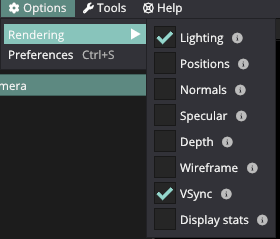
\includegraphics[width=0.5\textwidth]{images/menu_bar_options.png}
      \caption{Menu Bar Options}
      \label{fig:menu_bar_options}
    \end{figure}
  \item[Tools] 
    As well as rendering, \gls*{vmve} will provide many other tools such as
    audio, a built-in console, an editor etc. To facilitate this, a dedicated
    tools menu is included. Currently, this acts as a prototype but in the near
    future will contain a plethora of fully featured supporting tools.
    \begin{figure}[H]
      \centering
      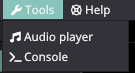
\includegraphics[width=0.25\textwidth]{images/menu_bar_tools.png}
      \caption{Menu Bar Tools}
      \label{fig:menu_bar_tools}
    \end{figure}
  \item[Help]
    Lastly, the help option is for users who need additional assistance whilst
    using the application. It provides information about the application but
    also, a link that redirects users to the documentation website for
    \gls*{vmve}
    \begin{figure}[H]
      \centering
      
\includegraphics[width=0.5\textwidth]{images/menu_bar_help.png}
      \caption{Menu Bar Help}
      \label{fig:menu_bar_help}
    \end{figure}
\end{description}


\subsubsection{Settings Window}

\begin{figure}[H]
  \centering
  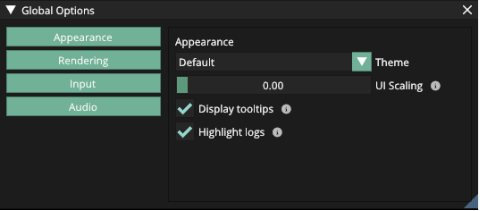
\includegraphics[width=\textwidth]{images/settings_window.png}
  \caption{Settings Window}
  \label{fig:settings_window}
\end{figure}

\subsubsection{Load Model Window} \label{load_model}

The load model window is accessed through \lstinline{File > Load Model} or by
pressing the \lstinline{Ctrl + L} shortcut. The window displays the file system
which contains a list of items and directories. The user can interact with this
in order to load a 3D model at runtime.
\begin{figure}[H]
  \centering
  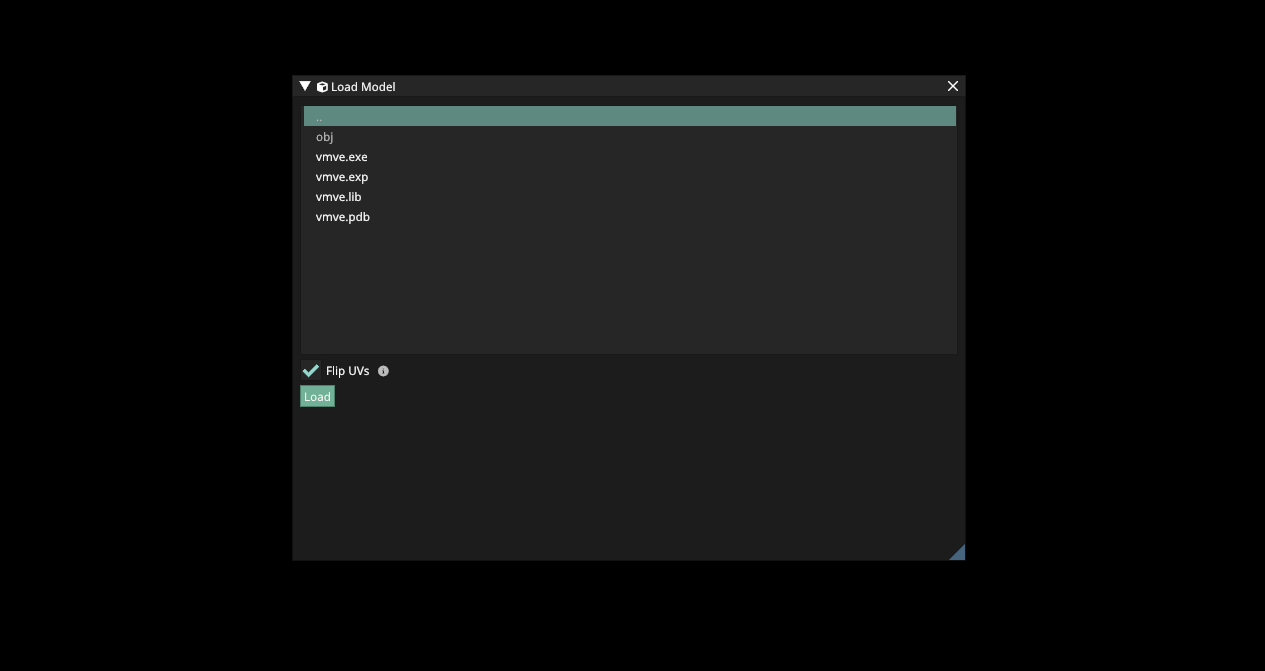
\includegraphics[width=\textwidth]{images/load_model_window.png}
  \caption{Load Model Window}
  \label{fig:load_model_window}
\end{figure}

If the 3D geometry file is detected to be encrypted then a modal window will
popup asking the user to enter the files encryption key and initialisation
vector. 
\begin{figure}[H]
  \centering
  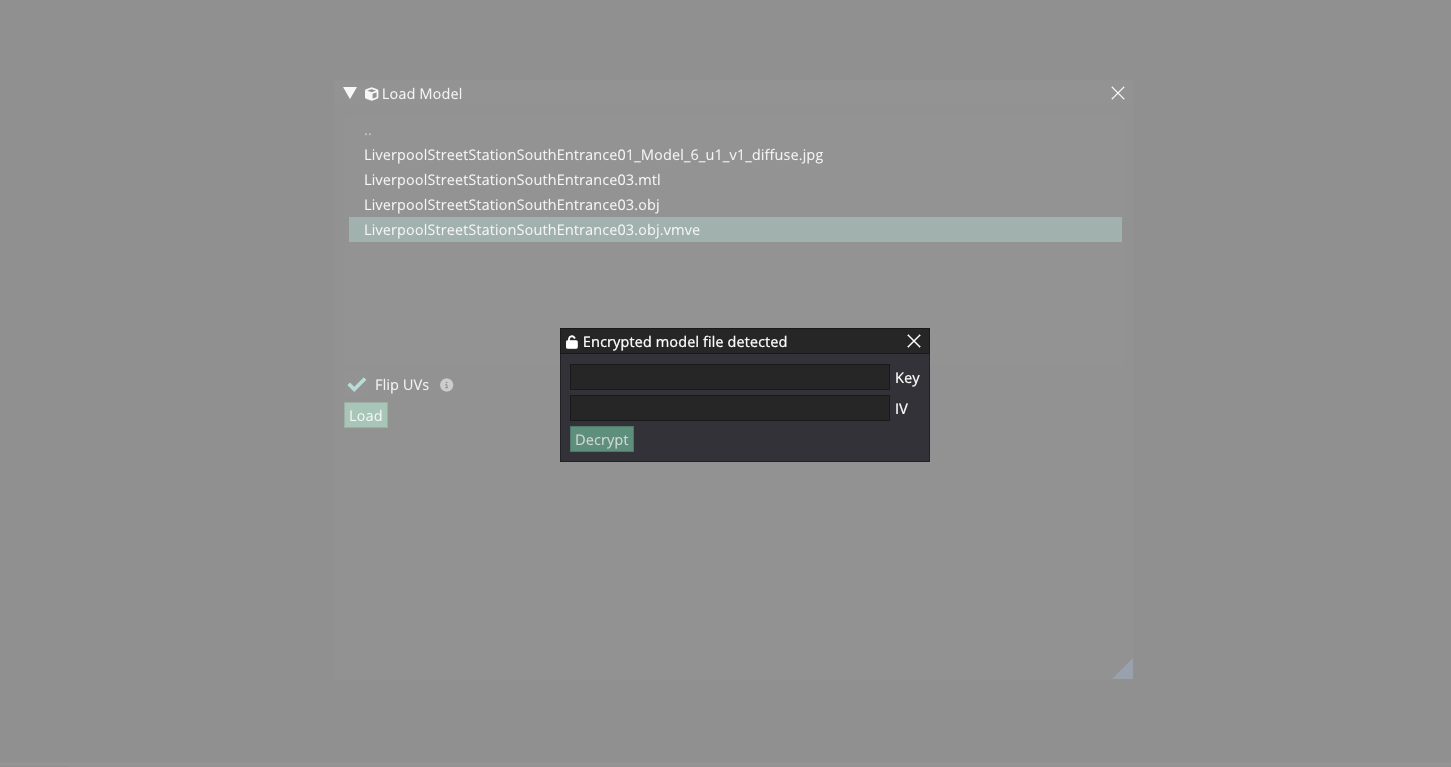
\includegraphics[width=\textwidth]{images/load_model_encrypted_window.png}
  \caption{Load Model Encrypted Window}
  \label{fig:load_model_encrypted_window}
\end{figure}

\subsubsection{Export Model Window}
The export window is responsible for encrypting and exporting models to the file
system. There are two key options when encrypting a model which are the
encryption mode and the length of the key. Users can change these options based
on their security requirements. The next step is to generate the key and
initialisation vector which can be performed by clicking on the ``Generate
key/iv'' button. Finally, the model can be encrypted.
\begin{figure}[H]
  \centering
  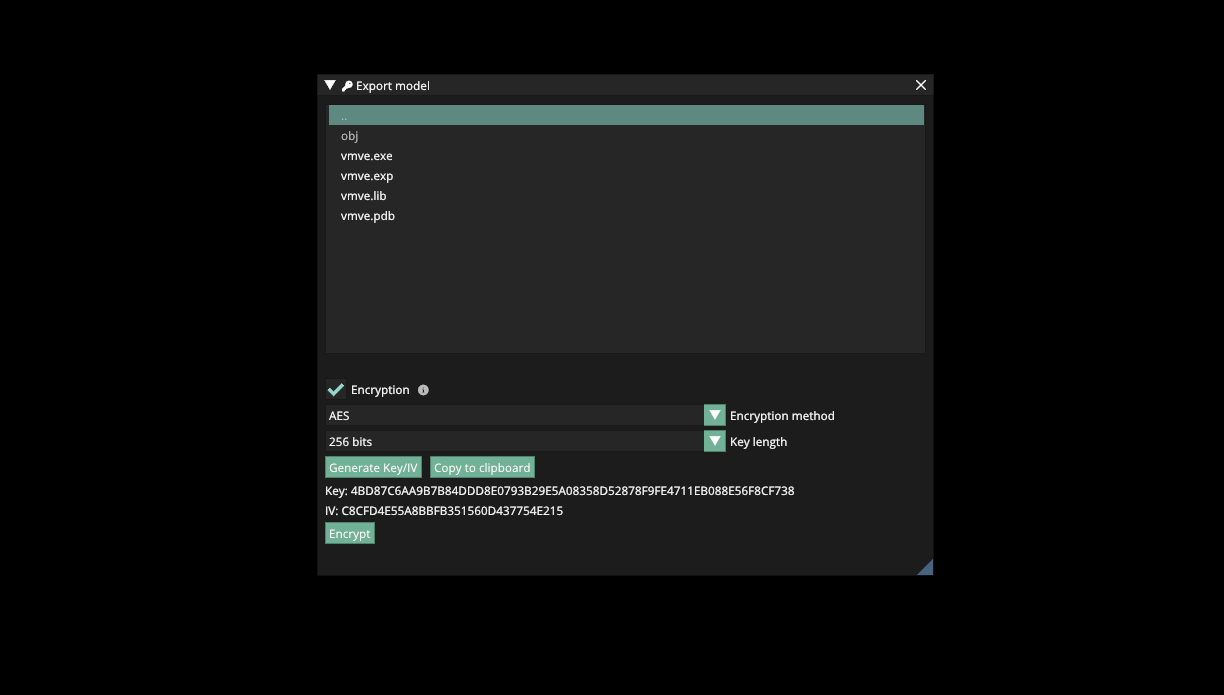
\includegraphics[width=\textwidth]{images/encryption_system.png}
  \caption{Export Model Window}
  \label{fig:encryption_window}
\end{figure}


\subsubsection{Global Panel}
The global panel contains application-wide information such as uptime and memory
usage. Additionally, camera information and properties can be configured here which
changes the way the virtual environment is rendered.

\begin{figure}[H]
  \centering
  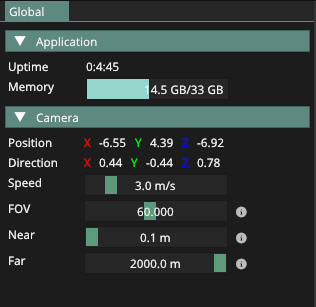
\includegraphics[width=0.5\textwidth]{images/global_panel.png}
  \caption{Global Panel}
  \label{fig:global_panel}
\end{figure}

\subsubsection{Entity Panel}
The main method of interacting with entities in the virtual environment is
through the entity panel. It contains a list of all loaded models in application
as well as the entities as shown in figure \ref{fig:entity_panel}. Below the
entity list is dedicated controls for a specifically selected entity. This
allows the user to manipulate the position, rotation and scale of an object in
the world.
\begin{figure}[H]
  \centering
  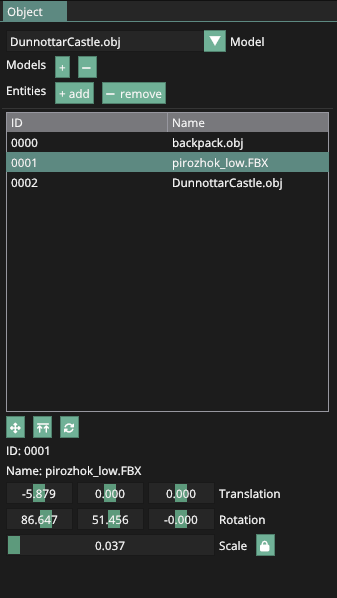
\includegraphics[width=0.5\textwidth]{images/entity_panel.png}
  \caption{Entity Panel}
  \label{fig:entity_panel}
\end{figure}

\subsubsection{Object gizmo}
An additional feature that is part of the user interface is the gizmo. This is a
visualisation of one of three operations is the main method of interaction that
a user has with an object and is used to specify the exact location and
orientation within the virtual environment. The operations are translation
(moving), rotation and scaling and can be seen in figure \ref{fig:gizmo}
respectively.
\begin{figure}[H]
  \centering
  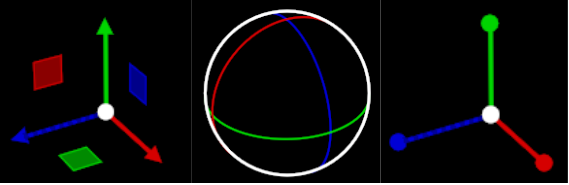
\includegraphics[width=\textwidth]{images/gizmo.png}
  \caption{Gizmo operations}
  \label{fig:gizmo}
\end{figure}

This functionality is implemented by taking the matrix transformation of an
object and feeding that information to ImGuizmo \cite{imguizmo}. It will then
perform the necessary mathematical calculations to convert from the objects
world space to screen space. In other words, no matter where in the virtual
environment the object is located, it will always be shown relative to the user's
screen. A small code snippet can be seen below \ref{fig:imguizmo_code} where
\(M\) represents the model in the \(MVP\) projection.


\begin{figure}[H]
  \centering
  \begin{lstlisting}[language=C++]
    const auto& operation = static_cast<ImGuizmo::OPERATION>(guizmo_operation);
    const auto& mode = ImGuizmo::MODE::WORLD;
    ImGuizmo::SetDrawlist();
    ImGuizmo::SetRect(x, y, viewport_x, viewport_y);
    ImGuizmo::Manipulate(view, proj, operation, mode, m);
  \end{lstlisting}
  \caption{ImGuizmo world to screen space}
  \label{fig:imguizmo_code}
\end{figure}

\subsection{Logging System}
Due to the relative complexity of the underlying application and the number of
moving components a logging system was developed to provide a clear
understanding of the current state of \gls*{vmve}. 

\begin{figure}[H]
  \centering
  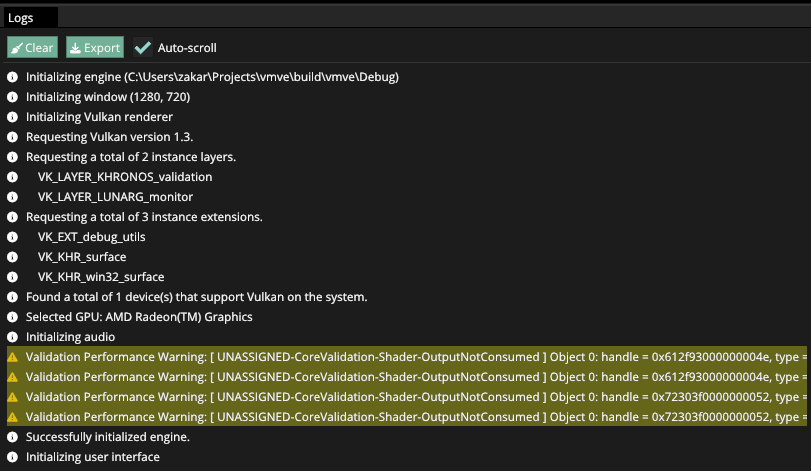
\includegraphics[width=\textwidth]{images/logging_window.png}
  \caption{Logging window}
  \label{fig:logging_window}
\end{figure}

Messages are stored in a data structure known as a ring buffer. This is a
fixed-size buffer where the start and end of the buffer are connected. In other
words, when the buffer becomes full, data stored at the start gets overwritten.

By default \gls*{vmve} allows for a maximum of 200 log messages before the
buffer becomes full. The underlying structure of this system can be seen in
figure \ref{fig:logging_system}.

\begin{figure}[H]
  \centering
  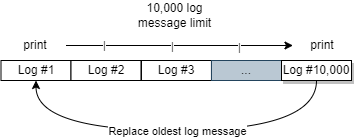
\includegraphics[width=\textwidth]{images/logging.png}
  \caption{Logging FIFO system}
  \label{fig:logging_system}
\end{figure}

The benefit of retaining log messages in memory as opposed to printing to the
console is that they can be used at a later time such as for the UI or being
saved to a file on disk.

\subsection{Encryption and Custom Model Format}
The simplicity of the Crypto++ library results in a relatively straightforward
function, shown in Figure \ref{fig:aes_encryption} which shows how a model is
encrypted using the AES algorithm.
\begin{figure}[H]
  \centering
  \begin{lstlisting}[language=C++]
    std::string encrypt_aes(const std::string& text, encryption_keys& keys, int key_size)
    {
        std::string encrypted_text;

        // Set key and IV to encryption mode
        CryptoPP::CBC_Mode<CryptoPP::AES>::Encryption encryption;
        encryption.SetKeyWithIV(
            reinterpret_cast<const CryptoPP::byte*>(keys.key.data()), 
            key_size, 
            reinterpret_cast<const CryptoPP::byte*>(keys.iv.data())
        );

        // Encrypt text
        CryptoPP::StringSource s(text, true, new CryptoPP::StreamTransformationFilter(encryption, new CryptoPP::StringSink(encrypted_text)));

        return encrypted_text;
    }
  \end{lstlisting}
  \caption{AES Encryption}
  \label{fig:aes_encryption}
\end{figure}


\subsubsection{Decryption validation}
When a model is being decrypted the system must check and ensure that the key
and iv being used match those originally used to encrypt it. Without this check
in place, the system will not know what the ``correct'' key and iv are.

As outlined during the design stage, the file header contains the encrypted key
and iv. When the user enters their specific key and iv as input parameters into
the decryption dialog box as shown in figure
\ref{fig:load_model_encrypted_window} in section \ref{load_model}, \gls*{vmve}
will first decrypt the header section and check if the input values match. If
successful, the application will then proceed to decrypt the data section and
then load the file. If however, this check fails, then the application will
throw an error and prevent the file from begin decrypted.




\subsection{Distribution}
The distribution is an important final step during the development of the
application which compiles and optimises the source code and makes the
application available for end users. Before compiling, the project configuration
is switched to ``Release'' mode as seen in figure \ref{fig:project_configuration}.

\begin{figure}[H]
  \centering
  
\includegraphics[width=\textwidth]{images/project_configuration.png}
  \caption{Project configuration}
  \label{fig:project_configuration}
\end{figure}

As mentioned in section \ref{development_environment}, the compiler used is
\gls*{msvc} and therefore, specific compiler flags are used. One such flag is
\lstinline{O2} which performs a series of optimisations during the compilation
phase which maximises speed such as frame-pointer omission, inline function
expansion, string deduplication, function-level linking and much more.

\subsubsection{Executable}
These optimations ensure that the resulting application has a small executable size
and performs efficiently. The resulting executable is named ``vmve.exe''.

\begin{figure}[H]
  \centering
  
\includegraphics[width=\textwidth]{images/executable.png}
  \caption{Executable}
  \label{fig:executable}
\end{figure}

\subsubsection{Versions}
\gls*{vmve} follows the major, minor and patch system of versioning and is used
as follows [Major].[Minor].[Patch]. The use of versions is important in
differentiating between \gls*{vmve} releases. Each new version of the application
comes with new features as well as bug fixes that aim to improve the software
over time. Due to the rapid development of new features and functionality,
backward compatibility cannot be guaranteed. The current official release of
\gls*{vmve} is v0.0.3.

\begin{figure}[H]
  \centering
  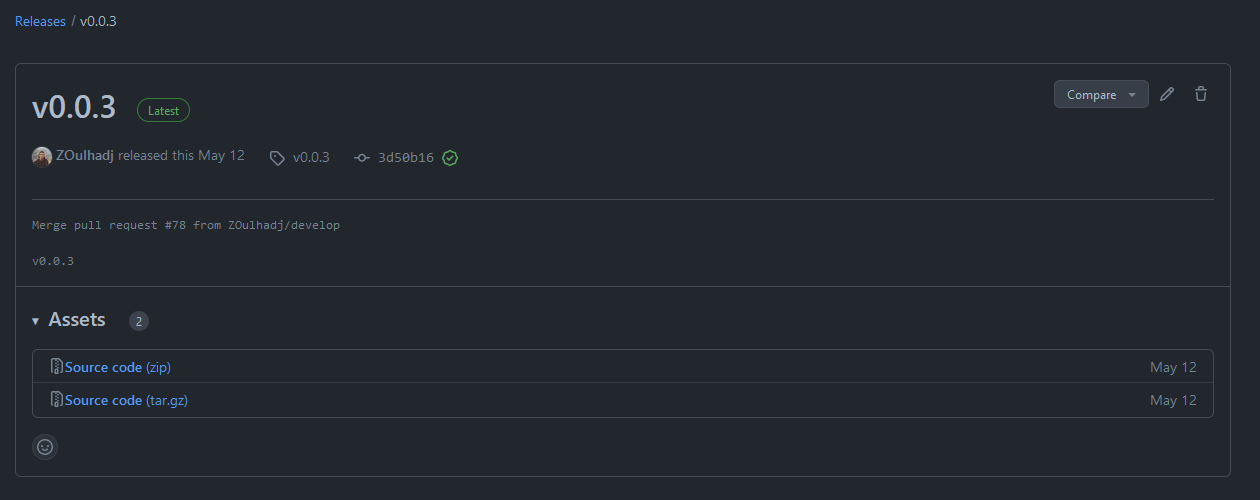
\includegraphics[width=\textwidth]{images/vmve_release.png}
  \caption{Latest release}
  \label{fig:latest_release}
\end{figure}

\subsubsection{Website}
Alongside the application, a website was created as a platform for easily
distributing the application. It includes a features section that showcases and
gives users a preview of the application through the use of images and videos.
Furthermore, a download link is provided giving users an easy way of obtaining
the executable without needing to understand the technicalities of GitHub as it
is designed with programmers in mind.

In regards to downloads, there are two types. The first is an active development
version which is regularly updated and acts as a beta release for versions that
have not yet been officially released. The second is current and past
\gls*{vmve} versions going all the back to the first official release (v0.0.1).

\begin{figure}[H]
  \centering
  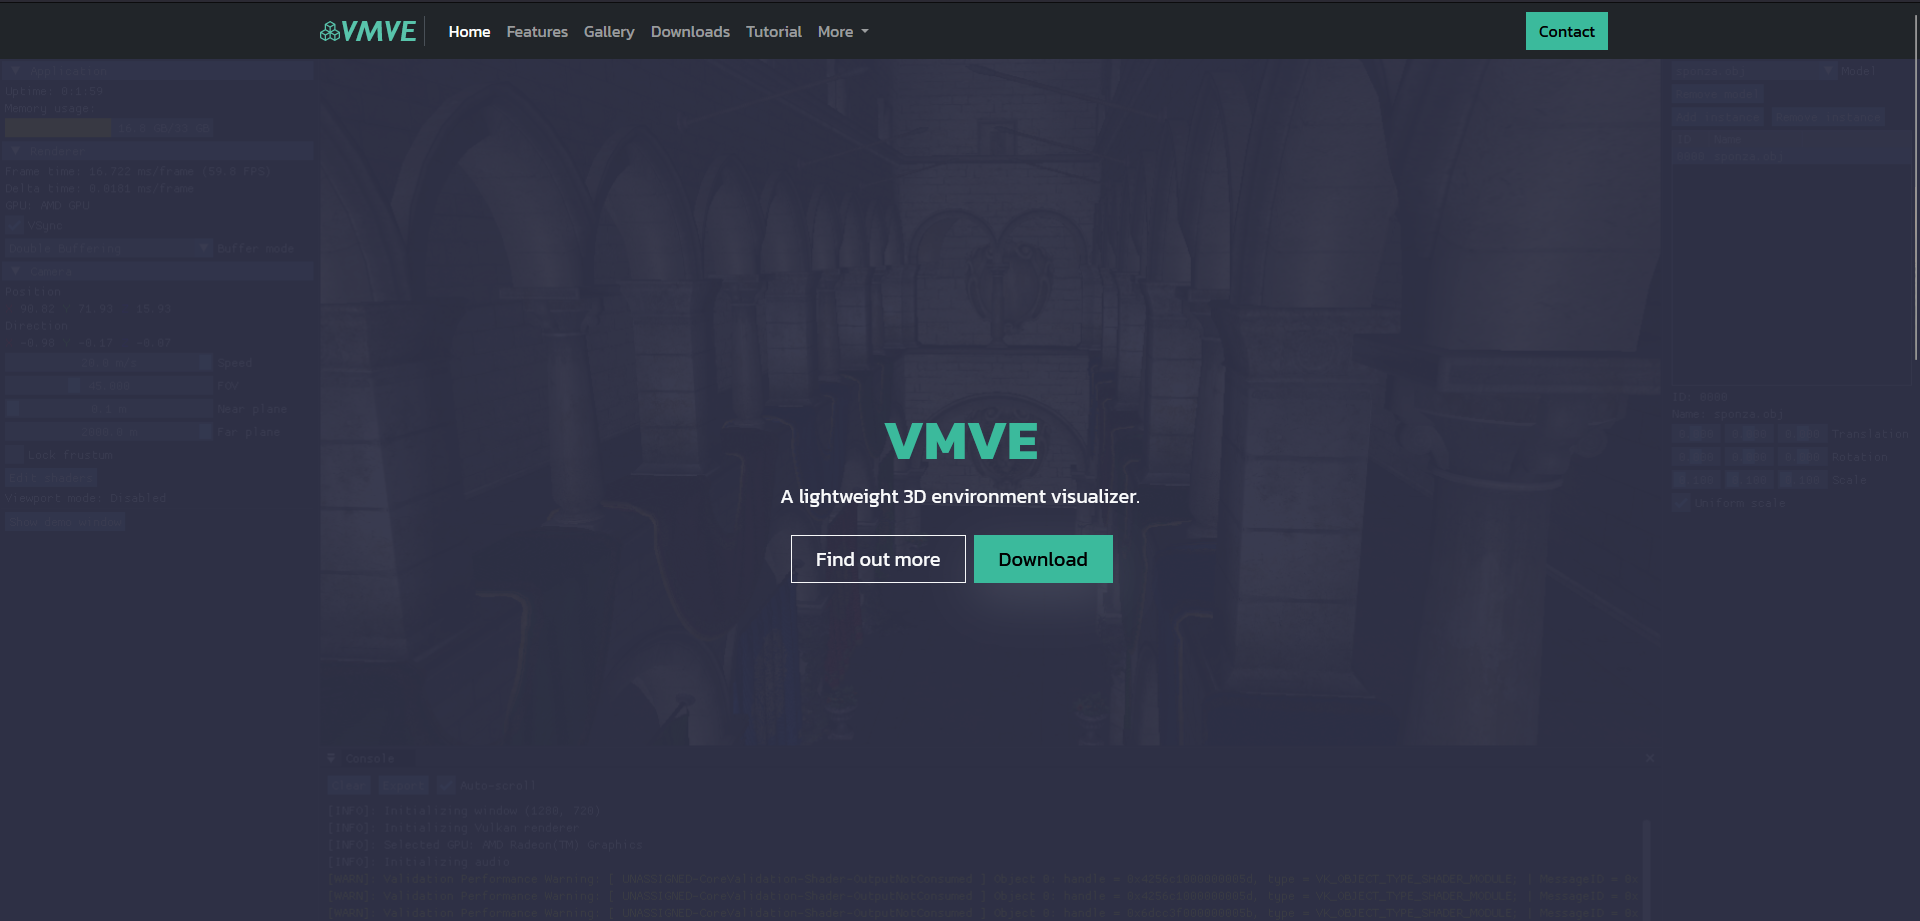
\includegraphics[width=\textwidth]{images/website.png}
  \caption{VMVE website}
  \label{fig:website}
\end{figure}


\subsubsection{Example models}
The \gls*{vmve} website provides an additional download link to six different
example models. These are provided by third parties (with appropriate credits)
and are corrected to ensure they can be loaded into \gls*{vmve} without any
issues. The purpose of these example models is to allow users to easily test the
application without needing to search the internet or create their own.

\begin{figure}[H]
  \centering
  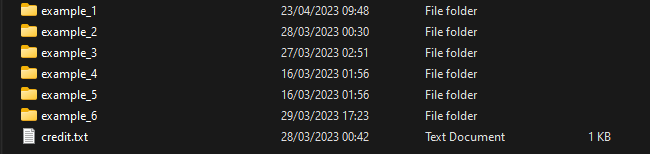
\includegraphics[width=\textwidth]{images/example_models.png}
  \caption{Example models}
  \label{fig:example_models}
\end{figure}

\subsubsection{Documentation}
In addition to a website, a documentation website was also created courtesy of
Read the Docs (\href{https://readthedocs.org}{https://readthedocs.org}). The
purpose of this site is to provide additional information about \gls*{vmve} and
also, provide an in-depth tutorial that aims to help users understand how to use
the application.

\begin{figure}[H]
  \centering
  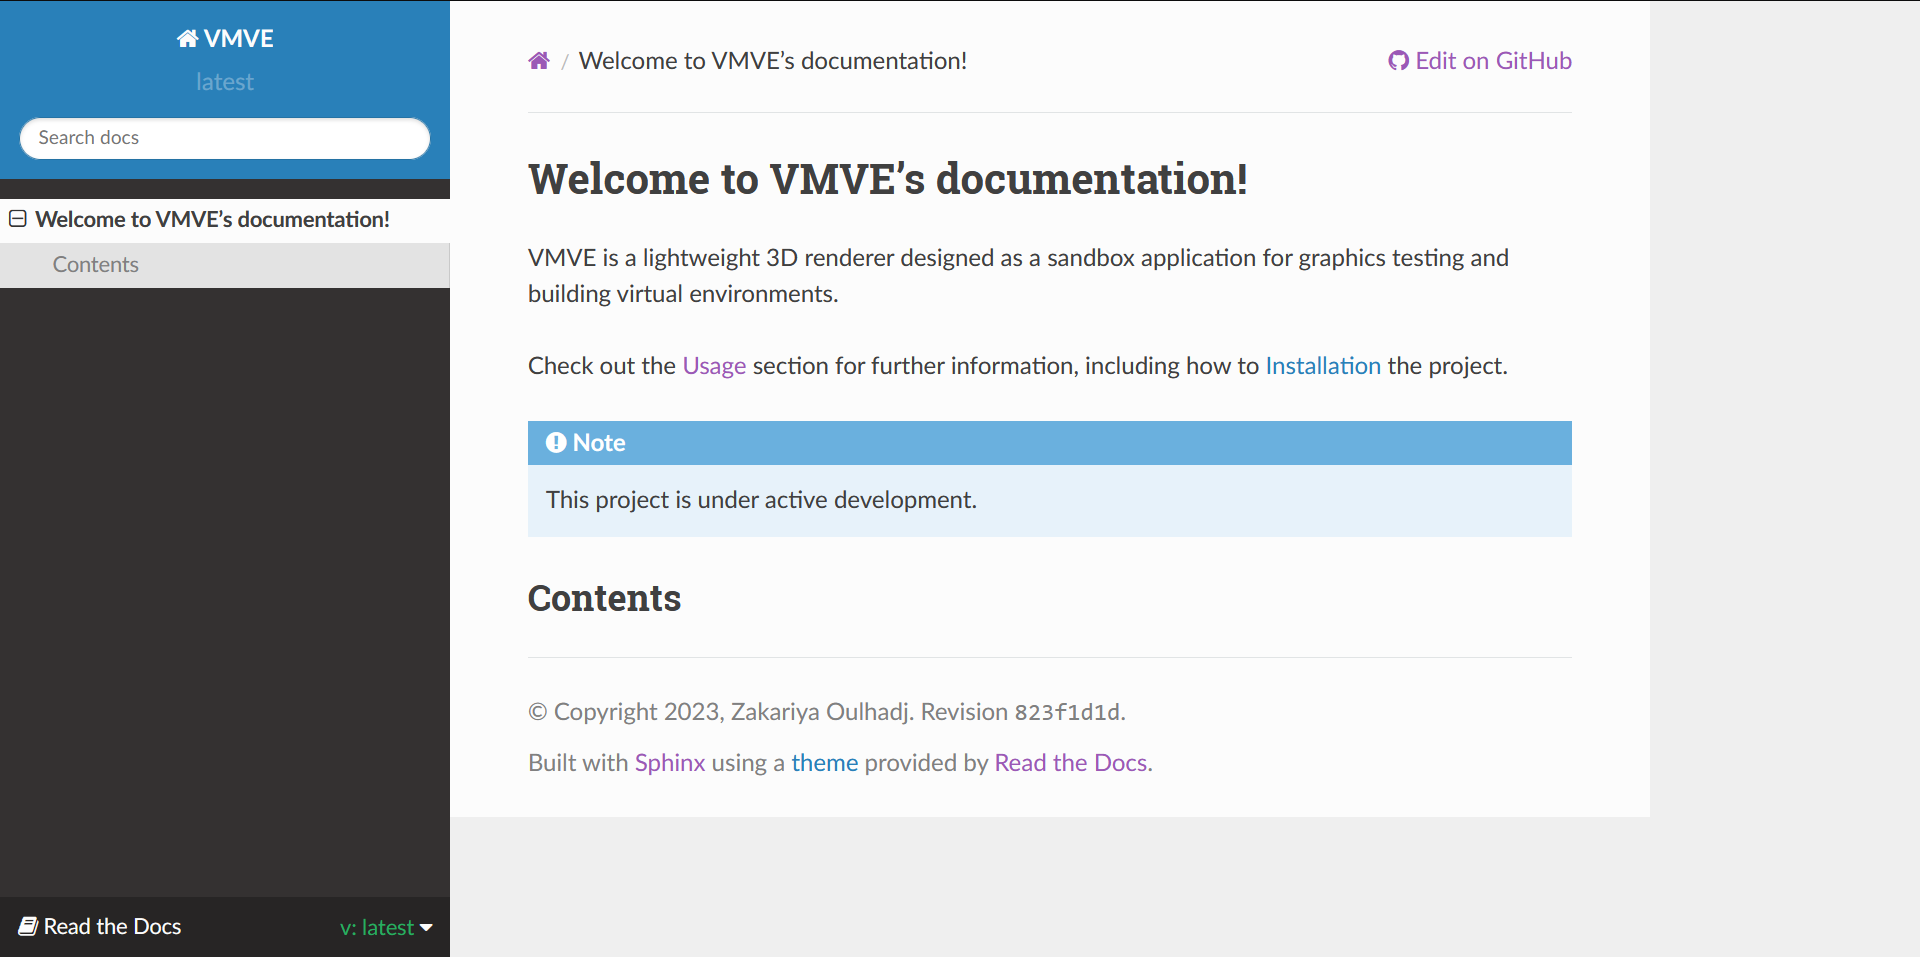
\includegraphics[width=\textwidth]{images/documentation.png}
  \caption{VMVE documentation}
  \label{fig:documentation}
\end{figure}


\subsection{Evaluation} \label{evaluation}
The completion of the project transitions into the evaluation stage where the
project is evaluated against the original goals and requirements in order to
judge if those requirements have been met. When evaluating the project there are
two distinct categories. The first is self-evaluation and the other is user
feedback.


\subsubsection{Distribution}
In hindsight, the most challenging aspect of the entire project was by far,
distribution and more specifically ensuring that \gls*{vmve} was able to run on
all supported systems as expected. Throughout the applications development,
there were points where \gls*{vmve} would work on the development machine,
however, throw an exception error on other systems. These inconsistencies paired
with the lack of reproducibility made these issues quite difficult to debug. The
majority of these inconsistencies between different systems occurred during the
initialisation stages. This would include creating the window, initialising the
renderer, initialising the UI, creating the audio system etc.

Some examples of these inconsistencies include the application crashing when
resizing the window, crashing if audio is disabled on a system as well as frame
stuttering.

\begin{figure}[H]
  \centering
  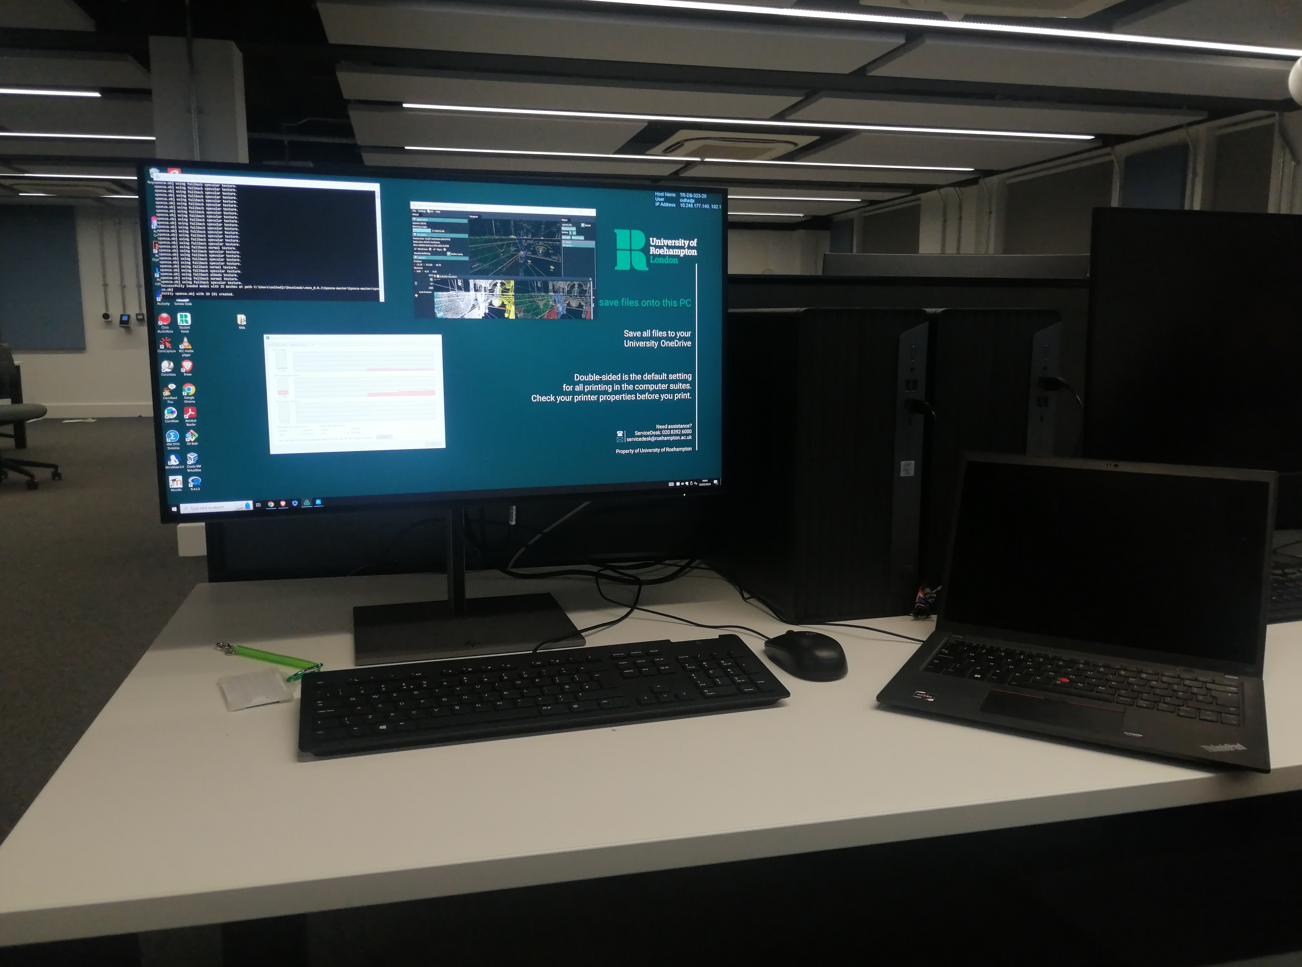
\includegraphics[width=\textwidth]{images/multiple_systems.png}
  \caption{Working on distribution}
  \label{fig:multiple_systems}
\end{figure}

During this part of development, the decision was made to design the logging
system so that all messages in the buffer would be stored and written to disk
before exiting. This allowed for unexpected crashes to be better understood as
the \lstinline{vmve_crash.txt} file could be analysed.

\subsubsection{Time Management}
Given the complexity of this project, it was vital to effectively manage time
during development and to ensure that all of the requirements of the project
could be met on time. Failure to correctly manage this workload would result in
key goals not being achieved and/or features not being implemented.

As mentioned in section \ref{project_management}, GitHub was chosen and has been
a highly effective tool throughout development regarding management and
distributing tasks. Over 50 different GitHub issues have been resolved such as
small user interface issues, implementation bugs and major structural changes.

Figure \ref{fig:commit_history} shows that a total of 357 commits were made over
the course of eight months. This includes the design and implementation stages
of the application.
\begin{figure}[H]
  \centering
  \includegraphics[width=\textwidth]{images/commit_history.png}
  \caption{Commit history}
  \label{fig:commit_history}
\end{figure}
    
\gls*{vmve} currently has 32 outstanding GitHub issues that have yet to be
resolved. These issues are not considered critical and do not hinder the project
in terms of meeting its original requirements. However, they are notable and
should be resolved soon.
\begin{figure}[H]
  \centering
  \includegraphics[width=\textwidth]{images/github_project.png}
  \caption{GitHub Issues Kanban}
  \label{fig:github_kanban}
\end{figure}

% \subsubsection{Hardware}
These tests were performed on the main development machine used throughout the
project which was a Thinkpad T14s Gen 3. The following list shown in figure
\ref{fig:development_machine} shows the laptop's specifications.

\begin{table}[H]
\centering
\begin{tabular}{|| c c ||} 
  \hline
  Component & Name \\ [0.5ex] 
  \hline\hline
  CPU & AMD Ryzen 7 Pro 6850U  \\ 
  GPU & Integrated \\
  RAM & 32GB DDR6 \\ 
  SSD & 1TB \\
  \hline
\end{tabular}
\caption{Development Machine}
\label{fig:development_machine}
\end{table}


\subsubsection{Performance}
Measuring the performance of \gls*{vmve} is another key aspect of evaluation that
ensures the original goals and requirements have been met. Two main aspects can
be measured which are compilation and runtime performance.

\begin{description}
  \item[Compilation] refers to the process of building the application in an offline
  setting. The speed at which the project is compiled directly affects the
  developer and subsequently the development of the project.
  \item[Runtime] refers to the performance of the application while it is running and
  its effects on the end users.
\end{description}

% \subsubsection{Compilation Performance}
A full clean build of \gls*{vmve} takes an average of 53.260 seconds using
Microsoft Visual Studio and the \gls*{cl} compiler. This includes the compilation
of the source code and precompiled headers. As the codebase for \gls*{vmve} grew
in both size and complexity, ensuring that compilation times were reasonable was
a vital aspect that had to be taken into consideration.

The main technique used for reducing compilation times was making use of a
\gls*{pch}. This is a header file (pch.h) that includes various header files such
as those from the standard library as well as external dependencies that are not
indented to change often. This is because a change to any of the included header
files will require a full precompiled header rebuild. The compiler compiles this
file once and is reused across compilations. This significantly reduces the
amount of work the compiler needs to perform since it does not have to recompile
the same sets of files needlessly each time.

This technique is done by including the ``pch.h'' header file at the top of each
translation unit (.cpp file) and before any other header file. This ensures that
the necessary types can be found for both header files and their corresponding
source files.

% \subsubsection{Runtime Performance}
\gls*{cpu} timing is primarily measured by calculating the difference in time at
two specific sections of the source code. Using C++ this can be easily achieved
by using the ``chrono'' library that allows for the duration to be calculated in
different time units such as nanoseconds, milliseconds, seconds and more. The
timing will be measured using milliseconds as that is the typical timescale for
applications such as \gls*{vmve}.

Using the aforementioned ``chrono'' library, the startup time for \gls*{vmve}
averages around 300ms in the distribution version of the application which is
calculated by taking away the time at the start of the initialisation from the
end of the initialisation.

The Microsoft Visual Studio \gls*{ide} allows us to further analyse this by
taking advantage of the built-in profiler which can be accessed by going to
\lstinline{Debug > Performance Profiler}. Figure
\ref{fig:vmve_startup_profiling} shows the ``flame graph'' that takes a snapshot
of the internal state of the application at runtime.

\begin{figure}[H]
  \centering
  \includegraphics[width=\textwidth]{images/startup_profiling_graph.png}
  \caption{\gls*{vmve} startup profiling}
  \label{fig:vmve_startup_profiling}
\end{figure}

What this shows us is that a large chunk of the initialisation is taken up by
the \lstinline{engine::configure_renderer} function and more specifically the
\lstinline{engine::create_shader} function which is responsible for compiling
the application shaders.

This can be taken a step further by expanding the hot code path which is what
Visual Studio refers to as slow code. Figure \ref{fig:vmve_slow_code_path} shows
the exact function that takes around 36\% of the total initialisation time.
\begin{figure}[H]
  \centering
  \includegraphics[width=\textwidth]{images/startup_profiling_slow_shader_compile.png}
  \caption{Profiling slow code path}
  \label{fig:vmve_slow_code_path}
\end{figure}

The question one might ask is, ``How can we improve this startup time?''.
Currently, \gls*{vmve} stores the shader source code as simple strings within a
header file called \lstinline{shader.h}. The main advantage of this is that
shaders can be combined with the executable rather than be in separate files.

The downside to this, however, is that the shader source is not in a precompiled
binary format, meaning that each time \gls*{vmve} runs, it must recompile the
shader files. 

In the future, this will need to be addressed and the system redesigned in such
a way that allows for shader files to be precompiled and bundled with the
executable at the same time eliminating the need to compile shader files and as
a result improving the startup time.


\begin{figure}[H]
  \centering
  \includegraphics[width=\textwidth]{images/visual_studio.png}
  \caption{Microsoft Visual Studio}
  \label{fig:visual_studio}
\end{figure}

\begin{figure}[H]
  \centering
  \includegraphics[width=\textwidth]{images/renderdoc.png}
  \caption{RenderDoc}
  \label{fig:renderdoc}
\end{figure}

\subsubsection{User Feedback}
Having conducted the evaluation, it is equally important to obtain feedback from
the stakeholders such as users. The users that tested the application were
predominantly other students. The process of obtaining this feedback was
separated into two stages.

The first was to measure how intuitive the user interface is which was achieved
by giving a user a set of instructions as seen in figure \ref{fig:instructions}
\textsuperscript{\textattachfile{attached_documents/user_feedback.xlsx}{\textcolor{skyblue}{file}}}.
A score would be given for each task based on how easily the user was able to
complete it.

\begin{figure}[H]
  \centering
  \includegraphics[width=\textwidth]{images/user_instructions.png}
  \caption{User feedback instructions }
  \label{fig:instructions}
\end{figure}

The second stage would obtain direct feedback from the users by presenting a
series of questions that would assess \glspl*{vmve} usability, performance and
overall user experience. This data was recorded using Google Forms and further
analysed to produce different sets of visualisations.

The bar chart below shows the results of an ease-of-use test that was conducted
between different users. The average ease of use score was 4.2. This indicates
that the majority of the users found the user interface to be suitable for users
regarding achieving their desired goals.

\begin{figure}[H]
  \centering
  \includegraphics[width=\textwidth]{images/bar_chart_usability.png}
  \caption{Usability bar chart}
  \label{fig:bar_chart_usability}
\end{figure}

Tom who gave the \gls*{vmve} an ease-of-use score of 3 said the following:
``\textit{Overall, the user interface is quite simple, however, I found that 
the shortcuts used throughout the application were not as easy to use as most
required the use of two hands}''. 

This highlights an important issue in terms of ergonomics between the
application and the user and as such will have to be addressed in the future.

Another test was conducted that asked users which of the main features of the
application required additional work and overall improvements. The pie chart in
figure \ref{fig:pie_chart_features} shows that lighting followed by performance
were the two most mentioned features.

\begin{figure}[H]
  \centering
  \includegraphics[width=\textwidth]{images/pie_chart_feature_improvements.png}
  \caption{Feature Improvements}
  \label{fig:pie_chart_features}
\end{figure}

Taylor, one of the users that tested the application said the following:
\textit{When displaying a single object VMVE can do this reasonably well without
any issues. However, when increasing the entity count so that there are many
objects in the scene, the performance of the application starts to drastically
lower}.

Based on how \gls*{vmve} has been initially developed, this makes sense as the
application does not make use of the many commonly found optimisations that are
required for rendering large quantities of objects. This also needs to be
addressed in future versions of the application so that usability is maintained,
and that \gls*{vmve} meets the demands and requirements of its users.

\subsection{Related Work}
% todo

\clearpage
\section{Conclusion} \label{conclusion}

\gls*{vmve} has been designed to be a platform in which users are provided with
easy to use 3D graphics tools without needing to know the complex implementation
details. This allows users to focus on their needs and requirements. The
application has been developed in line with the original aims and objectives
fulfilled with the primary aim of targeting students and trainees as an
education tool for the digital graphics industry. 

Although many of the original requirements have been met, the project as a whole
must be evaluated to analyse the various strengths and weaknesses at key stages
including requirements gathering, design, implementation and user feedback.

\subsection{Reflection}
This has been a long journey that has presented various challenges throughout
the development of \gls*{vmve}. Furthermore, a lot has been learned in different
areas.

\subsubsection{Time Management}
One of the major downsides that this project suffers from is the projects time
constraints. Given the relative complexity of the project, many of the features
implemented in \gls*{vmve} are quite rudimentary and serve as a basic prototype
that showcases the underlying technology and the potential future work that can
be undertaken.

\subsubsection{Design}
This project has also shown how important the requirements gathering and design
stages are. For example, the rendering architecture took longer to implement as 
certain aspects were not fully realised and designed ahead of time.

However, it's also important to recognise that in large projects such as this,
it can be difficult to fully define all the requirements as they may change over
time. Therefore, this needs to be taken into consideration for design stages in
future projects.

\subsubsection{Alternative Rendering API}
\gls*{vulkan} which as previously discussed is a low-level \gls*{gpu}
\gls*{api}. One of the major downsides to having chosen Vulkan as the \gls*{api}
of choice for this project was the significant amount of time that had to be
spent implementing the various rendering features due to how verbose and
technical the \gls*{api} is. The use of the API is only really beneficial if a
developer wants to make full use of the additional performance through the use
of multithreading, multiple command buffers and very specific memory allocation
requirements.

If given the choice, \gls*{vmve} would be rewritten to use a simpler \gls*{api}
such as DirectX11 or OpenGL as they provide the same functionality but with
significantly less work required. This would allow me to focus and spend more
time implementing the many other features required in such an application. In
the future, if the renderer's performance becomes an issue then the use of more
advanced \glspl*{api} could be reconsidered.

\subsubsection{Development Logs}
At key stages of the project's development, development logs i.e. videos were
recorded showcasing the state of development at that specific point in time. All
videos were uploaded and are hosted on the Zakariya Oulhadj YouTube channel
\url{https://www.youtube.com/@ZOulhadj}

\subsection{Future Work} \label{future_work} 
Looking forward to the future, several features need to be worked on and
implemented that aim to greatly increase \glspl*{vmve} usability and provide a
whole host of new features that benefit the key stakeholder groups.


\subsubsection{Multiple rendering APIs}
\gls*{vmve} currently only supports one rendering API which is Vulkan. As
discussed in the technology review section, Vulkan is officially supported on
Windows, Linux and macOS (through MoltenVK). However, to support additional
operating systems as well as hardware that does not support Vulkan, more
rendering APIs should be supported including DirectX12 and previous generation
APIs such as OpenGL and DirectX11 for increased compatibility.

\begin{figure}[H]
  \centering
  \includegraphics[width=\textwidth]{images/api_abstraction.png}
  \caption{Rendering API Abstraction}
  \label{fig:api_abstraction}
\end{figure}

\subsubsection{Frustum Culling}
Currently, VMVE sends all object data to the \gls*{gpu} to be processed and
rendered. The \gls*{gpu} then subsequently traverses each vertex to figure out if
it needs to be ``discarded''. This process is part of the graphics pipeline and
occurs for each vertex. As the complexity of both the scene and the objects
themselves increases, this starts to become a \gls*{gpu} intensive task and
results in increased \gls*{gpu} usage and lower performance.

To solve this, frustum culling must be implemented which is a rendering
optimisation in which objects not visible from the ``cameras point of view'' are
discarded completely and not sent to the GPU entirely. The term ``frustum'' refers
to the camera projection frustum which can be seen in figure
\ref{fig:frustum_culling} and ``Culling'' simply means discarding.

\begin{figure}[H]
  \centering
  \includegraphics[width=\textwidth]{images/frustum_culling.png}
  \caption{Frustum Culling \cite{frustum_culling}}
  \label{fig:frustum_culling}
\end{figure}


This technique significantly improves performance as each object in the world is
contained within a ``bounding box'' which is often a cube or a sphere
\ref{fig:bounding_boxes}. Then for each object, a check is performed against the
bounded box instead of the actual vertices. This allows for in the best case a
single check or at its worst 8 checks per object. This is far better than
needing to perform thousands of checks for all the vertices of an object.

\begin{figure}[H]
  \centering
  \includegraphics[width=\textwidth]{images/bounding_boxes.png}
  \caption{Bounding Boxes \cite{bounding_boxes}}
  \label{fig:bounding_boxes}
\end{figure}


\subsubsection{Spatial Acceleration Structures}
\gls*{vmve} only supports loading basic models however, in the future many other
features need to be implemented. One such feature is large-scale terrain as seen
in figure \ref{fig:quad_tree_terrain}.

\begin{figure}[H]
  \centering
  \includegraphics[width=\textwidth]{images/quad_tree_terrain.png}
  \caption{Large scale terrain}
  \label{fig:quad_tree_terrain}
\end{figure}

Currently, \gls*{vmve} would struggle to render such objects due to their
complexity in terms of the number of vertices required. For example, an area of
20x20km with a resolution of 1 meter would require 400 million vertices. Each
vertex, if packed efficiently could be 32 bytes each that includes positions (12
bytes), normals (12 bytes) and texture coordinates (8 bytes). In terms of
memory, this would require 12.8GB of data just for the terrain.

A common solution to this is implementing a type of spatial acceleration
structure also known as \gls*{lod}. These structures are designed as the name
suggests, to increase the speed of algorithms in the spatial domain including
images and environments.

A quadtree is a type of spatial acceleration structure that stores a
hierarchical collection of nodes that each represent a 2D area (and an octree in
the case of 3D). Figure \ref{fig:quad_tree} visualises a quadtree that shows
the resolution of each tile and how there are fewer tiles the further away from
the camera they are.

\begin{figure}[H]
  \centering
  \includegraphics[width=\textwidth]{images/quad_tree.png}
  \caption{Quad Tree visualisation}
  \label{fig:quad_tree}
\end{figure}

The benefit of using this technique is that the number of vertices is
significantly reduced saving on performance and memory usage.


\subsubsection{glTF Support}
Currently, the engine only really supports the \gls*{vmve} and OBJ model formats for
importing. The main issue with the OBJ file format is its size since the data is
stored in a text format which subsequently increases the assets file size. glTF
\cite{gltf} is a new model format by The Khronos Group that has many useful
features such as compression, binary representation, scene hierarchy and more.

\subsubsection{Cross Platform}
In contrast to the project's initial proposal which was the support multiple
\glspl*{os}, Windows is the only \gls*{os} that \gls*{vmve} officially supports due
to the time constraints for this project. 

Going beyond the final deadline, \gls*{vmve} should add cross-platform support
which would greatly benefit the application as it would increase flexibility in
terms of which \glspl*{os} its able to run on and subsequently, increase the
potential user base. Implementing such functionality would require significant
changes to the underlying architecture of the application such as implementing
opaque types for structures that have different implementations depending on the
\gls*{os} being used. Additionally, a different build system would have to be
used that is cross-platform such as CMake \cite{cmake} or Premake \cite{premake}.

\subsubsection{Networking Support}
\gls*{vmve} is a virtual environment editor and as such can be significantly
improved by adding support for networking. The idea is that there would be a
server running which would keep track of the virtual world and multiple clients
via \gls*{vmve} would be able to connect and interact with the environment
simultaneously.

This would allow for greater efficiency and speed up various tasks. For example,
multiple users could work together to construct a virtual environment in
preparation for scientific research which would otherwise have taken much longer
had only one user worked on it.

\subsubsection{File Format/Encryption}
\gls*{vmve} supports both the AES encryption standard by default. The application
should also include additional encryption algorithms such as Diffie-Helm and
RC6. This would provide users with greater flexibility in terms of how their
assets are encrypted as well as varying levels of encryption strength/methods
based on the user's encryption requirements.

Another feature that will need to be added to the application is related to the
custom model format and the ability to store and encrypt other types of data.
Currently, the encrypted data stores just the vertices and their corresponding
information. The downside to this is that assets such as textures are still
required to be located alongside the ``.vmve'' file since the format does not
support textures.

In the future, \gls*{vmve} should be able to store textures so that users can be
left with a single asset file that includes all the information, similar to how
the glTF model format supports the ``.glb'' binary file. This would
significantly increase the user's experience since assets files would become
easier to manage.

\subsubsection{Runtime memory protection}
One of the major flaws present is the lack of security that prevents a user from
maliciously altering the memory of the application during runtime so that
encrypted models can be accessed without the need for a valid key or iv.

This can be achieved using applications such as Cheat Engine which provides
users with a set of tools for analysing memory addresses, offsets and values
that can also be manipulated \cite{cheat_engine}. For example, an attacker could
alter the boolean statement that checks if the key and iv being inputted are
valid. Doing so would force the application to go ahead and decrypt a model.

This will need to be addressed in future versions of \gls*{vmve} so that digital
assets remain secure for all users. A possible alternative implementation would
involve the use of symmetric and asymmetric encryption as well as techniques
designed specially to prevent runtime memory manipulation.

\subsubsection{Version Control}
In regards to the \gls*{vcs} architecture, a potential change that can be done is
to add a third branch called ``Beta''. The purpose of this branch would be to
release relatively stable yet unfinished features to users. This would allow
users to use new features and test them before an official version is released.
Overall, this would reduce the number of bugs in final versions and be
beneficial to users who are keen on using recently developed features. Figure
\ref{fig:futurebrancharch} shows how the \gls*{vcs} architecture could look like
with the addition of a ``Beta'' branch.

\begin{figure}[H]
  \centering
  \includegraphics[width=\textwidth]{images/future_branch_design.png}
  \caption{Potential future git branch design}
  \label{fig:futurebrancharch}
\end{figure}

\subsubsection{Reduce Library Dependencies}
\gls*{vmve} makes use of several libraries which allows specific functionality to
be added quickly. This is ideal given the project's time constraints and
requirements. However, going forward the aim will be to reduce the number of
external libraries being used.

This will provide various benefits such as less reliance on external code,
faster compilation times as only functionality that is required will be
implemented and generally finer control of the code that \gls*{vmve} is built on
top of.

\subsubsection{Accessibility}
Another aspect that needs to be addressed soon is improved accessibility. The
application includes some features that address this such as icons, a tutorial,
documentation as well as additional information. However, some of the features
that \gls*{vmve} does not include is taking into account color blindness and
text-to-speech. The reason for this is that these are more complex topics and
required additional time and research to ensure a proper implementation is
released.

Another task that must be considered is localisation. \gls*{vmve} only supports
the English language and has no way of adapting to other languages. Therefore,
the internal structure of the application must be redesigned to allow for
other languages to be added and thus, improving accessibility.



\clearpage
\bibliographystyle{IEEEtran}
\bibliography{IEEEabrv, refs}

\clearpage
\section{Appendices}
The appendices may be referenced throughout the report which provides additional
information or access to important documents.

\subsection{Supporting Documents} \label{supporting_documents}
\begin{description}
  \item[\textattachfile{attached_documents/milestone_1.pdf}{\textcolor{skyblue}{Milestone 1}}] 
    Project initiation document for milestone 1.
  \item[\textattachfile{attached_documents/milestone_2_signed.pdf}{\textcolor{skyblue}{Milestone 2}}]
    Project proposal document for milestone 2.
  \item[\textattachfile{attached_documents/mid_project_review.pdf}{\textcolor{skyblue}{Milestone 3}}]
    Mid-term project review document for milestone 3.
  \item[\textattachfile{attached_documents/meetings.docx}{\textcolor{skyblue}{Meetings}}]
    A complete log of all meetings held during the project.
  \item[\textattachfile{report.tex}{\textcolor{skyblue}{Source}}]
    The source code to this latex document.
\end{description}

\subsection{GitHub} \label{github}
The \gls*{vmve} project is hosted on GitHub as a private repository which can be
found at the following link: \url{https://github.com/ZOulhadj/vmve/}

\subsection{Rendering API History} \label{rendering_api_appendix}
One of the core aspects of \gls*{vmve} is making use of the underlying hardware and
more specifically the GPU (Graphics Processing Unit) which will be primarily
used for rendering. Taking advantage of the GPUs hardware capabilities requires
low-level access to the hardware and is not as straightforward as one would
hope. To understand why, we must first understand how Graphics Processing Units
function.

There are different types of GPUs such as dedicated or onboard, different
architectures including AMDs RDNA \cite{RDNA} or NVIDIAs ADA \cite{ADA} as well
as various capabilities that differ between hardware vendors. An application
attempting to target GPUs would need to consider this including having access to
the GPU drivers (Low-level software that allows a specific piece of hardware to
function). Oftentimes, software drivers are trade secrets that companies do not
want freely available. Given the complexity and variations of modern
\glspl*{gpu} this is simply not feasible.

Companies from across different industries solved this issue by creating
an open, non-profit consortium in the early 2000s called The Khronos Group. This
organisation develops, publishes and maintains standards for different areas
but most notably for 3D Graphics and Computation. Companies follow these 
standards when developing software allowing for interoperability across
hardware. As of 2023, The Khronos Group actively maintains 16 different
standards. Out of all those standards, there are two which are the most
suitable for \gls*{vmve}, OpenGL and \gls*{vulkan}.

OpenGL and \gls*{vulkan} are two types of rendering APIs that are designed based on
The Khronos Group specifications. When attempting to provide graphics support
for a particular \gls*{gpu}, hardware vendors follow the OpenGL and/or \gls*{vulkan}
specifications when implementing their drivers. For applications, a
\gls*{api} is provided allowing for direct control of the \gls*{gpu}.

\gls*{vmve} could support both OpenGL and \gls*{vulkan} however, due to the vast
amount of work required to accomplish this as well as the project's time
constraints this is simply not feasible. Instead, both need to be evaluated to
choose one.


\subsection{Camera Transformation}
\begin{figure}[H]
  \centering
  \begin{lstlisting}[language=C++]
    // Construct M (model)
    glm::mat4 m = glm::mat4(1.0f);
    m = glm::translate(m, world_position);   
    m = glm::rotate(m, radians, rotation_axis); 
    m = glm::scale(m, scale_amount);

    // Construct V (view)
    glm::mat4 v = glm::lookAt(camera_position, camera_direction, camera_up);

    // Construct P (projection)
    glm::mat4 p = glm::perspective(field_of_view, aspect_ratio, near, far);

    // Construct MVP
    glm::mat4 mvp = p * v * m; // Order is important

  \end{lstlisting}
  \caption{Complete MVP example}
  \label{fig:local_to_world_appendix}
\end{figure}


\end{document}

% end of the document